\chapter{Graphs}\label{ch:Graphs}

\newthought{In chapter \ref{ch:Relations}  we represented a relation with a graph.  In this chapter
we discuss a more general notion of a  graph.}

\section{Some Graph Terminology} There is a lot of new vocabulary to absorb concerning graphs!
For this chapter, a {\bfseries graph} will consist of a number of points (called {\bfseries vertices}) (singular: {\bfseries vertex}) together with
lines (called {\bfseries edges}) joining some (possibly none, possibly all) pairs of vertices. Unlike the graphs of earlier chapters, we will not allow an edge from a vertex back to itself (so no loops allowed), we will not allow multiple edges between vertices, and the edges will not be directed (there will be no edges with arrowheads on one or both ends).  All of our graphs will have a finite vertex sets, and consequently a finite number of edges. Graphs are typically denoted by an uppercase letter such as $G$ or $H$.


If you would like a formal definition:
 a {\bfseries {graph}}, $G$ consists of a set of vertices $V$ and a set $E$ of edges, where
an edge $t\in E$ is written as an unordered pair of vertices $\{u,v\}$, (in other words, a set consisting of two \underbar{different} vertices). We say that the edge $t= \{u,v\}$ has {\bfseries endpoints} $u$ and $v$, and that the edge $t$ 
is {\bfseries {incident}} to both $u$ and $v$. The vertices $u$ and $v$ are {\bfseries {adjacent}} when there is an edge with endpoints $u$ and $v$; otherwise they are not adjacent.  Such a formal definition is necessary, but a more helpful way to think of a graph is as a diagram.

Here is an example of a graph $G$ with vertex set $\{a,b,c,d,e\}$ illustrating these concepts.

\begin{center}
 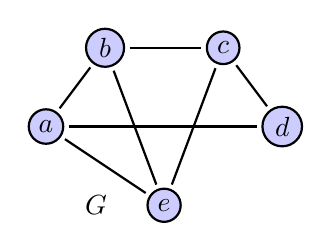
\begin{tikzpicture}[node distance=0.5cm,
                       thick,main node/.style={circle,fill=blue!20,draw,outer sep=2pt,inner sep=2pt}
                      ] 
  \node[main node] (a) at (-1.5,0) {$a$};
  \node[main node] (b) at (-0.75,1.00) {$b$};
  \node[main node] (c) at (0.75,1.00) {$c$};
  \node[main node] (d) at (1.5,0) {$d$};
  \node[main node] (e) at (0,-1.00) {$e$};
  \node (G) at (-0.866,-1.000) {$G$};  
  \path%
   (a) edge [left] node {} (b)
   (a) edge [left] node {} (d)
   (a) edge [left] node {} (e)
   (b) edge [left] node {} (c)
   (b) edge [left] node {} (e)
   (c) edge [left] node {} (d)
   (c) edge [left] node {} (e);
 \end{tikzpicture}
\end{center}

The placement of the vertices in a diagram representing a graph is (within reason!) not important.
Here is another diagram of that same graph $G$. 


\begin{center}
 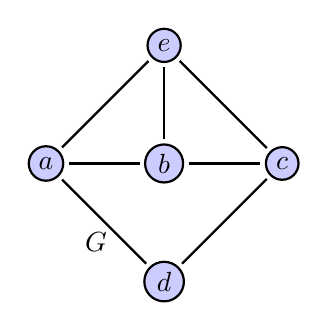
\begin{tikzpicture}[node distance=0.5cm,
                       thick,main node/.style={circle,fill=blue!20,draw,outer sep=2pt,inner sep=2pt}
                      ] 
  \node[main node] (a) at (-1.5,0.00) {$a$};
  \node[main node] (b) at (0.00,0.00) {$b$};
  \node[main node] (c) at (1.50,0.00) {$c$};
  \node[main node] (d) at (0.00,-1.50) {$d$};
  \node[main node] (e) at (0.00, 1.50) {$e$};
  \node (G) at (-0.866,-1.000) {$G$};  
  \path%
   (a) edge [left] node {} (b)
   (a) edge [left] node {} (d)
   (a) edge [left] node {} (e)
   (b) edge [left] node {} (c)
   (b) edge [left] node {} (e)
   (c) edge [left] node {} (d)
   (c) edge [left] node {} (e);
 \end{tikzpicture}
\end{center}

In this diagram, we again have vertex set  $a,b,c,d,e$, and edges \\
$\{a,b\}, \{b,c\},\{c,d\},\{a,d\},\{a,e\},\{b,e\},\{c,e\}$, and that is all that matters. 
It is a good idea to draw a diagram that is easy to understand! In particular, while any curve can be used to represent an edge between two vertices, whenever it is reasonable, edges are normally drawn as straight lines. 
The vertices $b$ and $e$ are adjacent and the vertices $b$ and $d$ are not adjacent. The vertices $a$ and $c$ are not adjacent since there is no edge $\{a,c\}$.  If we use $s$ to denote the  edge joining $b$ to $c$, then $s$ has endpoints $b$ and $c$, and $s$ is incident to $b$ and $c$. 



Applying the {\it a-picture-is-worth-a-thousand-words} principle, for the small graphs we will be working with, a graph diagram is generally the easiest way to represent a graph.



\subsection{Representing a graph in a computer}

There are two standard ways to represent a graph in computer memory, both involving matrices (in other words, tables of numbers). The matrices are of a special type called  $0,1$-matrices since the table entries will all be either $0$ or $1$. 

{\underbar{\bfseries Adjacency matrix}}: If there are $n$ vertices in the graph $G$, the adjacency matrix is an $n$ by $n$ square table of numbers. The rows and columns of the table are labeled with the symbols used to name the vertices. The names are used in the same order for the rows and columns, so there are $n!$ possible labelings. Often there will be some {\it natural} choice of the order of the labels, such as alphabetic or numeric order. The entries in the table are determined as follows: the matrix entry with row label $x$ and column label $y$ is $1$ if $x$ and $y$ are adjacent, and $0$ otherwise. 


{\underbar{\bfseries Incidence matrix}}: Suppose the graph $G$ has $n$ vertices and $m$ edges. The table 
will have $n$ rows, labeled with the names of the vertices,  and $m$ columns labeled with the edges. Which of the $n!m!$ possible orderings of these labelings has to be specified in some way.  The entry in the row labeled with vertex 
$u$ and column labeled with edge $e$ is $1$ if $e$ is incident with $u$, and $0$ otherwise. Since every edge is incident to exactly two vertices, every column of the incidence matrix will have exactly two $1$'s.


\begin{exmp}\label{example01}
 Let $G$ have vertex set $\{u_1,u_2,u_3,u_4,u_5\}$ and edges  $\{u_1,u_2\}, 
 \{u_2,u_3\},\{u_3,u_4\},\{u_4,u_5\},\{u_5,u_1\}, \{u_5,u_3\}$. A graphical  representation of  $G$
 is 
 \begin{center}
 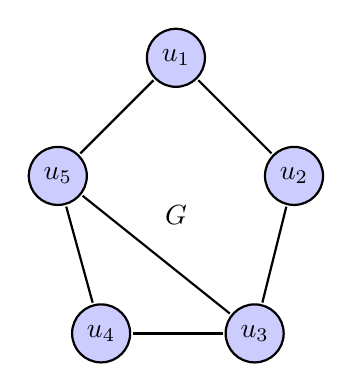
\begin{tikzpicture}[node distance=1cm,
                               thick,main node/.style={circle,fill=blue!20,draw,outer sep=1pt}
                              ]        
             \node[main node] (1) at (0,0) {$u_5$};
             \node[main node] (2) at (1.5,1.5) {$u_1$};
             \node[main node] (3) at (3,0) {$u_2$};
             \node[main node] (4) at (2.5,-2.00) {$u_3$};
             \node[main node] (5) at (0.55,-2.00) {$u_4$};
             \node (G) at (1.50,-0.50) {$G$};          
             \path%
               (1) edge node [right] {} (2)  %{} is where the edge value would go
               (2) edge [right] node {} (3)
               (3) edge [right] node {} (4)
               (4) edge [left] node {} (5)
               (5) edge [left] node {} (1)
               (1) edge [left] node {} (4);
         \end{tikzpicture}
\end{center}


 Here are the  adjacency matrix $A_G$, and the  incidence matrix $M_G$ of $G$
 using the vertices and edges in the orders given above.
 
 \[
  A_G=\left[
   \begin{matrix}
    0&1&0&0&1 \\ 
    1&0&1&0&0 \\ 
    0&1&0&1&1 \\ 
    0&0&1&0&1 \\ 
    1&0&1&1&0
   \end{matrix}
  \right]
  \qquad
  M_G=\left[
  \begin{matrix}
    1&0&0&0&1&0\\
    1&1&0&0&0&0 \\ 
    0&1&1&0&0&1 \\ 
    0&0&1&1&0&0 \\
    0&0&0&1&1&1
   \end{matrix}
  \right]
 \]
 
\end{exmp} 

\section{An Historical Interlude: The origin of graph theory}

Unlike most areas of mathematics, it is possible to point the a specific person as the creator of graph theory and a specific problem that  led to its creation. On the following pages  the {\it Seven Bridges of K\"onigsberg} problem  and the graph theoretic approach to a solution provided by Leonard Euler in $1736$ is described. 

The notion of a graph discussed in the article is a little more general that the graphs we will be working with in the chapter. To model the bridge problem as a graph, Euler allowed multiple edges between vertices. In modern terminology, graphs with multiple edges are called {\bfseries multigraphs}.   

While we are on the topic of extensions of the definition of a graph, let's also mention the 
case of graphs with {\it loops}. Here we allow an edge to connect a vertex to itself, forming a 
loop. Multigraphs with loops allowed are called {\bfseries pseudographs}. Another generalization
of the basic concept of a graph is {\bf hypergraph}: in a hypergraph, a single edge is  allowed to
connect not just two, but any number of vertices. 

Finally, for all these various types of graphs, we can consider the {\bfseries directed} versions in which the edges are given arrowheads on one or both ends to indicate the permitted direction of travel along that edge. 

In the following article, multigraphs are employed. {\it But after the article we will again refer only to graphs with no multiple edges and and no loops.}



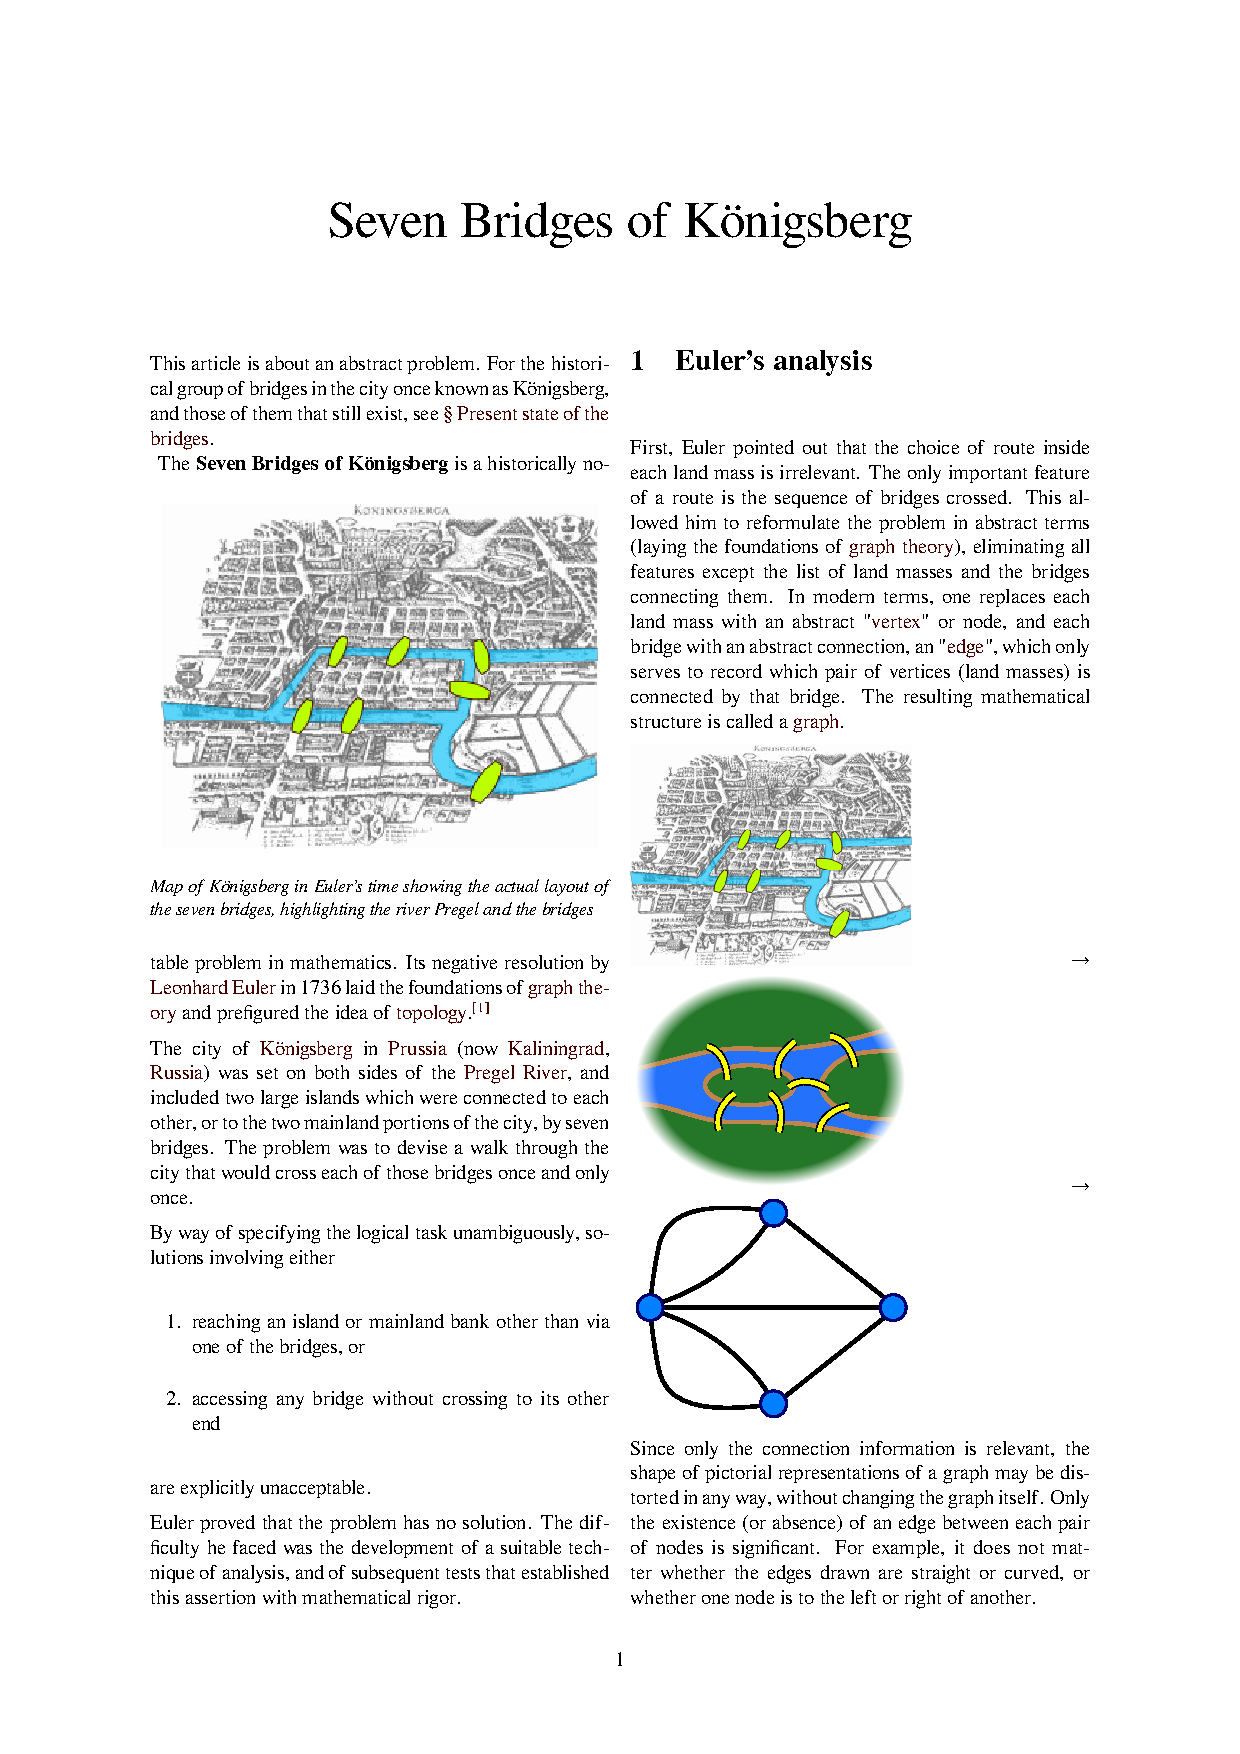
\includepdf[pages=-,offset= 0 0]{Chapters/SBridgesofK.pdf}

\section{The First Theorem of Graph Theory}

For a vertex
$v$ in a graph  we denote the number of edges incident to $v$ as the {\bfseries {degree}}
of $v$, written as $deg(v)$. For example, consider the graph

\begin{center}
 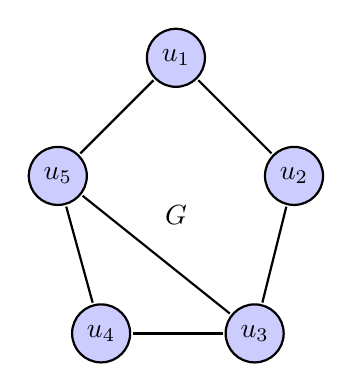
\begin{tikzpicture}[node distance=1cm,
                               thick,main node/.style={circle,fill=blue!20,draw,outer sep=1pt}
                              ]        
             \node[main node] (1) at (0,0) {$u_5$};
             \node[main node] (2) at (1.5,1.5) {$u_1$};
             \node[main node] (3) at (3,0) {$u_2$};
             \node[main node] (4) at (2.5,-2.00) {$u_3$};
             \node[main node] (5) at (0.55,-2.00) {$u_4$};
             \node (G) at (1.50,-0.50) {$G$};          
             \path%
               (1) edge node [right] {} (2)  %{} is where the edge value would go
               (2) edge [right] node {} (3)
               (3) edge [right] node {} (4)
               (4) edge [left] node {} (5)
               (5) edge [left] node {} (1)
               (1) edge [left] node {} (4);
         \end{tikzpicture}
\end{center}

Vertices $u_1, u_2, u_4$ each have degree $2$, while $deg(u_3)$ and $deg(u_5)$ are each $3$.
The list of the degrees of the vertices of a graph is called the {\bfseries degree sequence} of the graph.
The degrees are traditionally listed in increasing order. So the degree sequence of the graph $G$ above is $2,2,2,3,3$.

The following theorem is usually referred to as the {\it First Theorem of Graph Theory}


\begin{thm}
 The sum of the degrees of the vertices of a graph equals twice the number of edges. In particular, the sum of the degrees is even.
\end{thm}
\begin{proof}
 Notice that, when adding the degrees for the vertices,
each edge will contribute two to the total, once for each end.
So the sum of the degrees is twice the number of edges. 
\end{proof}

For example, in the graph $G$ above, there are $6$ edges, and the sum of the degrees of the vertices is $2+2+2+3+3= 12 = 2(6)$.


\begin{corollary}
 A graph must have an even number of vertices of odd degree.
 \end{corollary}
 \begin{proof}
Split the vertices into two groups: the vertices with even degree and the vertices with odd degree. The sum of all the degrees is even, and the sum of all the even degrees is also even. That implies that the sum of all the odd degrees must also be even. Since an odd number of odd integers adds up to an odd integer, it must be that there is an even number of odd degrees.
\end{proof}

\section{A Brief Catalog of Special Graphs} 
 

It is convenient to have names for some particular types of graphs that occur frequently. 

For $n\geq 1$, $K_n$ denotes the graph with $n$ vertices where every pair of vertices
 is adjacent.  $K_n$ is the {\bfseries {complete graph}} on $n$ vertices. So $K_{n}$ is the largest possible graph with $n$ vertices in the sense that it has the maximum possible number of edges.
 \begin{marginfigure}
 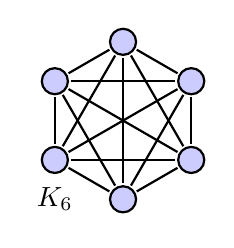
\begin{tikzpicture}[node distance=3cm,
                        thick,main node/.style={circle,fill=blue!20,draw,outer sep=1pt}
                       ]    
      \node[main node] (1) at (0.000,1.000) {};
      \node[main node] (2) at (0.866,0.500) {};
      \node[main node] (3) at (0.866,-0.500) {};
      \node[main node] (4) at (0.00,-1.000) {};
      \node[main node] (5) at (-0.866,-0.500) {};
      \node[main node] (6) at (-0.866,0.500) {};      
       \node (K6) at (-0.866,-1.000) {$K_{6}$};    
      \path%
        (1) edge node [right] {} (2)  %{} is where the edge value would go
        (1) edge [right] node {} (3)
        (1) edge [right] node {} (4)
        (1) edge [left] node {} (5)
        (1) edge [left] node {} (6)
        (2) edge [left] node {} (3)
        (2) edge [left] node {} (4)
        (2) edge [right] node {} (5)
        (2) edge [right] node {} (6)
        (3) edge [right] node {} (4)
        (3) edge [left] node {} (5)
        (3) edge [left] node {} (6)
        (4) edge [left] node {} (5)
        (4) edge [left] node {} (6)
        (5) edge [right] node {} (6);
 \end{tikzpicture}
 \end{marginfigure}

 
  For $n\geq 3$, $C_n$ denotes the graph with $n$ vertices, $v_1,...,v_n$, where 
each vertex in that list is adjacent to the vertex that follows it and $v_n$ is adjacent to $v_1$. The graph  $C_n$ is called the {\bfseries {$n$-cycle}}. The graph $C_3$ is called a {\bfseries triangle}.
 
  \begin{marginfigure}
 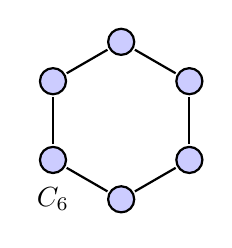
\begin{tikzpicture}[node distance=3cm,
                        thick,main node/.style={circle,fill=blue!20,draw,outer sep=1pt}
                       ]    
      \node[main node] (1) at (0.000,1.000) {};
      \node[main node] (2) at (0.866,0.500) {};
      \node[main node] (3) at (0.866,-0.500) {};
      \node[main node] (4) at (0.00,-1.000) {};
      \node[main node] (5) at (-0.866,-0.500) {};
      \node[main node] (6) at (-0.866,0.500) {};      
       \node (C6) at (-0.866,-1.000) {$C_{6}$};    
      \path%
        (1) edge node [right] {} (2)  %{} is where the edge value would go        
        (2) edge [left] node {} (3)        
        (3) edge [right] node {} (4)        
        (4) edge [left] node {} (5)       
        (5) edge [right] node {} (6)
        (6) edge [left] node {} (1);
 \end{tikzpicture}
 \end{marginfigure}

 For $n\geq 2$, $L_n$ denotes the {\bfseries {$n$-link}}. An $n${-}link is a row of $n$ vertices with each vertex adjacent to the following vertex.
  Alternatively, for $n\geq 3$, an $n${-}link is produced by erasing one edge from an $n${-}cycle. 
  
  \begin{marginfigure}
 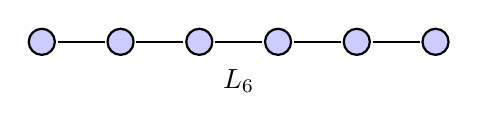
\begin{tikzpicture}[node distance=3cm,
                        thick,main node/.style={circle,fill=blue!20,draw,outer sep=1pt}
                       ]    
      \node[main node] (1) at (-2,-1.0) {};
      \node[main node] (2) at (-1,-1.0) {};
      \node[main node] (3) at (0,-1.0) {};
      \node[main node] (4) at (1,-1.0) {};
      \node[main node] (5) at (2,-1.0) {};
      \node[main node] (6) at (3,-1.0) {};      
       \node (L6) at (.5,-1.500) {$L_{6}$};    
      \path%
        (1) edge node [right] {} (2)  %{} is where the edge value would go        
        (2) edge [left] node {} (3)        
        (3) edge [right] node {} (4)        
        (4) edge [left] node {} (5)       
        (5) edge [right] node {} (6);       
 \end{tikzpicture}
 \end{marginfigure}

 For $n\geq 3$, $W_n$ denotes the {\bfseries {$n$-wheel}}. To form $W_n$ add one vertex
 to $C_n$ and make it adjacent to every other vertex. Notice that the $n$-wheel has $n+1$ vertices.
 
 \begin{marginfigure}
 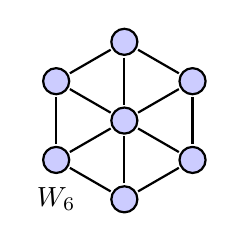
\begin{tikzpicture}[node distance=3cm,
                        thick,main node/.style={circle,fill=blue!20,draw,outer sep=1pt}
                       ]    
      \node[main node] (1) at (0.000,1.000) {};
      \node[main node] (2) at (0.866,0.500) {};
      \node[main node] (3) at (0.866,-0.500) {};
      \node[main node] (4) at (0.00,-1.000) {};
      \node[main node] (5) at (-0.866,-0.500) {};
      \node[main node] (6) at (-0.866,0.500) {};   
      \node[main node] (7)  at (0.00, 0.00) {};
       \node (W6) at (-0.866,-1.000) {$W_{6}$};    
      \path%
        (1) edge node [right] {} (2)  %{} is where the edge value would go        
        (2) edge [left] node {} (3)        
        (3) edge [right] node {} (4)        
        (4) edge [left] node {} (5)       
        (5) edge [right] node {} (6)
        (6) edge [left] node {} (1)
        (1) edge node [right] {} (7)         
        (2) edge [left] node {} (7)        
        (3) edge [right] node {} (7)        
        (4) edge [left] node {} (7)       
        (5) edge [right] node {} (7)
        (6) edge [left] node {} (7);

 \end{tikzpicture}
 \end{marginfigure}
 
  For $n\geq 1$, the {\bfseries {$n$-cube}}, $Q_n$, is the graph whose vertices are labeled with the $2^{n}$ bit  strings
 of length $n$. The unusual choice of names for the vertices is made so it will be easy to describe the edges in the graph: two vertices are adjacent provided their labels differ in exactly one bit. Except for $n = 1,2,3$ it is not easy to draw a convincing diagram of $Q_{n}$. The graph $Q_{3}$ can be drawn so it looks like what you would probably draw if you wanted a picture of a 3-dimensional cube. In the graph below, there is a vertex placed at each of the eight corners of the $3${-}cube labeled with the name of the vertex.
 
 \begin{center}
 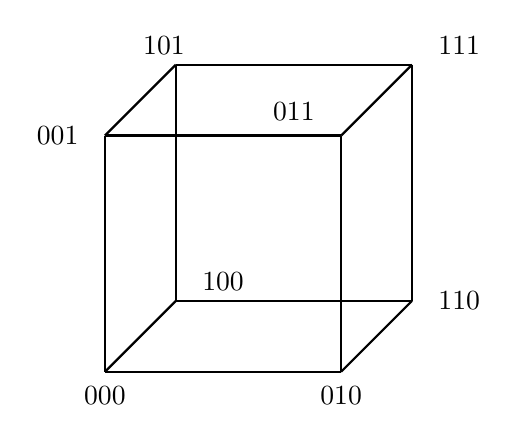
\begin{tikzpicture}[thick,scale=3]
    \coordinate (A1) at (0, 0);
    \node at (0, -.1)  {$000$};
    \coordinate (A2) at (0, 1);
    \node at (1, -.1)  {$010$};
    \coordinate (A3) at (1, 1);
    \node at (1.5, .3)  {$110$};
    \coordinate (A4) at (1, 0);
     \node at (.5, .38)  {$100$};
    \coordinate (B1) at (0.3, 0.3);
    \node at (-.2,1 )  {$001$};
    \coordinate (B2) at (0.3, 1.3);
    \node at (.25, 1.38)  {$101$};
    \coordinate (B3) at (1.3, 1.3);
    \node at (1.5, 1.38)  {$111$};
    \coordinate (B4) at (1.3, 0.3);
     \node at (.8, 1.1)  {$011$};

    \draw (A1) -- (A2);
    \draw (A2) -- (A3);
    \draw (A3) -- (A4);
    \draw (A4) -- (A1);

    \draw (A1) -- (B1);
    \draw (B1) -- (B2);
    \draw (A2) -- (B2);
    \draw (B2) -- (B3);
    \draw (A3) -- (B3);
    \draw (A4) -- (B4);
    \draw (B4) -- (B3);
    \draw (B1) -- (B4);
    
\end{tikzpicture}    

\end{center}
 
  A graph is {\bfseries {bipartite}} if it is possible to split the vertices into two subsets, let's call them $T$ and $B$ for top and bottom, so that all the edges  go from a vertex in one of the subsets to a vertex in the other subset.
  
  For example, the graph below is a bipartite graph  with  $T = \{a,b,c\}$ and $B = \{d,e,f,g\}$. 
  
 \begin{center} 
  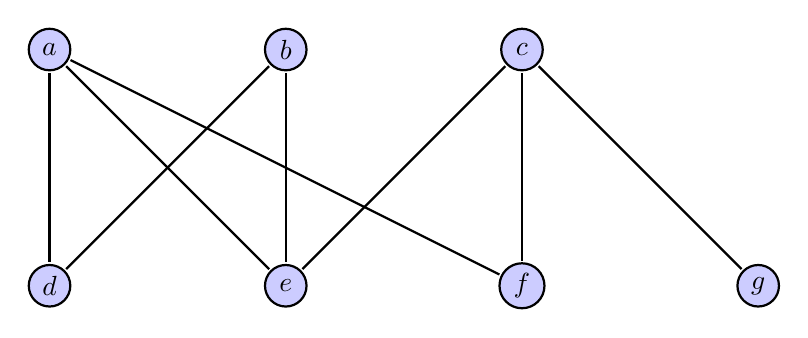
\begin{tikzpicture}[node distance=1cm,
                      thick,main node/.style={circle,fill=blue!20,draw,outer sep=1pt,
                      inner sep=2pt,minimum size=15pt}
                     ]           
   \node[main node] (a) at (0.0,0.0) {$a$};
   \node[main node] (b) at (3.0,0.0) {$b$};
   \node[main node] (c) at (6.0,0.0) {$c$};
   \node[main node] (d) at (0.0,-3.0) {$d$};
   \node[main node] (e) at (3.0,-3.0) {$e$};       
   \node[main node] (f) at (6.0,-3.0) {$f$};
   \node[main node] (g) at (9.0,-3.0) {$g$};
   \path%
     (a) edge node [right] {} (d)  %{} is where the edge value would go
     (a) edge [left] node {} (e)    
     (a) edge [left] node {} (f)
     (b) edge [left] node {} (e)
     (b) edge [left] node {} (d)
     (c) edge [left] node {} (e)
     (c) edge [left] node {} (f)
     (c) edge [left] node {} (g);
\end{tikzpicture}
\end{center}
  
   
  
  

    
    If $T$  has $m$ vertices and $B$ has $n$ vertices, and every vertex in $T$ is adjacent to every vertex in $B$,  the graph  is called the {\bfseries {complete bipartite graph}}, and it is denoted by $K_{m,n}$. Here is the graph $K_{3,4}$:
    
     \begin{center} 
  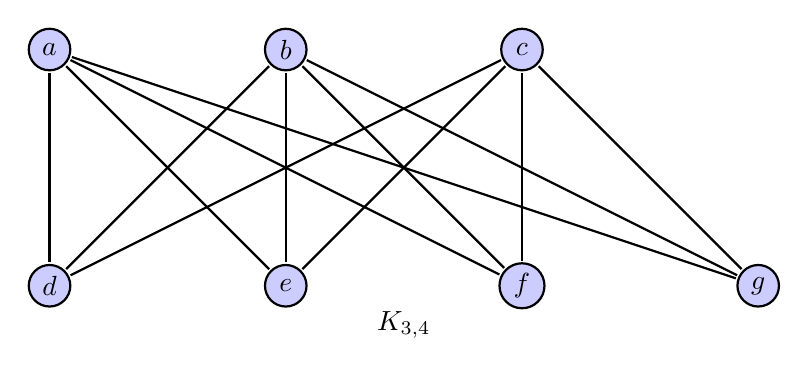
\begin{tikzpicture}[node distance=1cm,
                      thick,main node/.style={circle,fill=blue!20,draw,outer sep=1pt,
                      inner sep=2pt,minimum size=15pt}
                     ]           
   \node[main node] (a) at (0.0,0.0) {$a$};
   \node[main node] (b) at (3.0,0.0) {$b$};
   \node[main node] (c) at (6.0,0.0) {$c$};
   \node[main node] (d) at (0.0,-3.0) {$d$};
   \node[main node] (e) at (3.0,-3.0) {$e$};       
   \node[main node] (f) at (6.0,-3.0) {$f$};
   \node[main node] (g) at (9.0,-3.0) {$g$};
   \node (K34) at (4.5,-3.5) {$K_{3,4}$}; 
   
   \path%
     (a) edge node [right] {} (d)  %{} is where the edge value would go
     (a) edge [left] node {} (e)    
     (a) edge [left] node {} (f)
     (a) edge [left] node {} (g)
     (b) edge node [right] {} (d) 
     (b) edge [left] node {} (e)    
     (b) edge [left] node {} (f)
     (b) edge [left] node {} (g)
     (c) edge node [right] {} (d)
     (c) edge [left] node {} (e)    
     (c) edge [left] node {} (f)
     (c) edge [left] node {} (g);
     
\end{tikzpicture}
\end{center}
  
It is not always obvious if a graph is bipartite or not when looking at a diagram. For example  the square 
\begin{center} 
  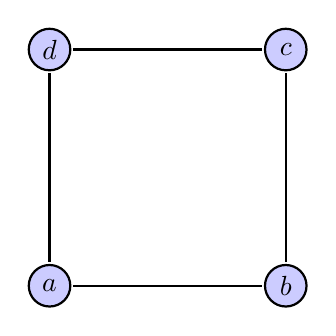
\begin{tikzpicture}[node distance=1cm,
                      thick,main node/.style={circle,fill=blue!20,draw,outer sep=1pt,
                      inner sep=2pt,minimum size=15pt}
                     ]           
   \node[main node] (a) at (0.0,0.0) {$a$};
   \node[main node] (b) at (3.0,0.0) {$b$};
   \node[main node] (c) at (3.0,3.0) {$c$};
   \node[main node] (d) at (0.0,3.0) {$d$};
   
   
   \path%
     (a) edge node [right] {} (b)  %{} is where the edge value would go
     (b) edge [left] node {} (c)    
     (c) edge [left] node {} (d)
     (d) edge [left] node {} (a);     
\end{tikzpicture}
\end{center}

is bipartite since the graph can be redrawn as

\begin{center} 
  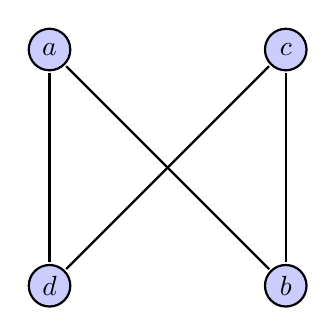
\begin{tikzpicture}[node distance=1cm,
                      thick,main node/.style={circle,fill=blue!20,draw,outer sep=1pt,
                      inner sep=2pt,minimum size=15pt}
                     ]           
   \node[main node] (d) at (0.0,0.0) {$d$};
   \node[main node] (b) at (3.0,0.0) {$b$};
   \node[main node] (c) at (3.0,3.0) {$c$};
   \node[main node] (a) at (0.0,3.0) {$a$};
   
   
   \path%
     (a) edge node [right] {} (b)  %{} is where the edge value would go
     (b) edge [left] node {} (c)    
     (c) edge [left] node {} (d)
     (d) edge [left] node {} (a);     
\end{tikzpicture}
\end{center}

so we can see the graph is actually $K_{2,2}$ in disguise.




\section{Graph isomorphisms}

The graphs $G$ and $H$ are obviously really the same except for the labels used for the vertices.

\begin{center}
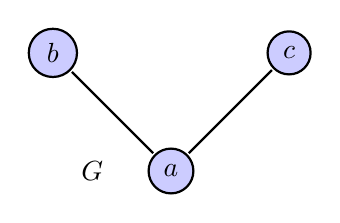
\begin{tikzpicture}[node distance=1cm,
                               thick,main node/.style={circle,fill=blue!20,draw,outer sep=1pt}]     
             \node[main node] (1) at (0,0) {$a$};
             \node[main node] (2) at (1.5,1.5) {$c$};
             \node[main node] (3) at (-1.5,1.5) {$b$};
             \node (G) at (-1,0) {$G$};          
             \path%
               (1) edge node [right] {} (2)  %{} is where the edge value would go
               (1) edge [right] node {} (3);
         \end{tikzpicture}
         \hskip 50pt
         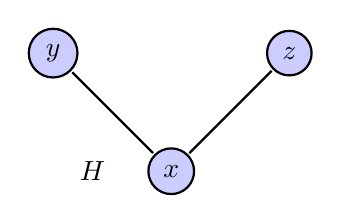
\begin{tikzpicture}[node distance=1cm,
                                 thick,main node/.style={circle,fill=blue!20,draw,outer sep=1pt}]
             \node[main node] (1) at (0,0) {$x$};
             \node[main node] (2) at (1.5,1.5) {$z$};
             \node[main node] (3) at (-1.5,1.5) {$y$};
             \node (H) at (-1,0) {$H$};          
             \path%
               (1) edge node [right] {} (2)  %{} is where the edge value would go
               (1) edge [right] node {} (3);                       
           \end{tikzpicture}
\end{center}

This idea of {\it sameness} (the official phrase is  the graphs $G$ and $H$ are {\bfseries isomorphic}) for graphs is defined as follows: Two graphs $G$ and $H$ are isomorphic provided we can relabel the vertices of one of the graphs using the labels of the other graph in such a way that the two graphs will have exactly the same edges. As you can probably guess, the notion of isomorphic graphs is an equivalence relation on the collection of all graphs.

In the example above, if the vertices of $H$ are relabeled as $a\to x$ (meaning replace $x$ with $a$), and 
$b\to y$, $c\to z$, then the graph $H$ will have edges $\{a,b\}$ and $\{a,c\}$ just like the graph $G$. So we have proved $G$ and $H$ are isomorphic graphs. The set of  replacement rules, $a\to x$, $b\to y$, $c\to z$, is called
an {\bfseries isomorphism}.

The graph $G$ is also isomorphic to the $3$-link $L_{3}$: 
\begin{center}
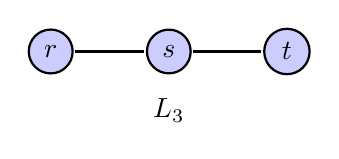
\begin{tikzpicture}[node distance=1cm,
                               thick,main node/.style={circle,fill=blue!20,draw,outer sep=1pt}]     
             \node[main node] (1) at (0,0) {$s$};
             \node[main node] (2) at (-1.5,0) {$r$};
             \node[main node] (3) at (1.5,0) {$t$};
             \node (L3) at (0,-.75) {$L_{3}$};          
             \path%
               (1) edge node [right] {} (2)  %{} is where the edge value would go
               (1) edge [right] node {} (3);
         \end{tikzpicture}
\end{center}    

In this case, an isomorphism is $a\to s$, $b\to r$, $c\to t$. 

On the other hand, $G$ is certainly not isomorphic to the $4$-cycle, $C_{4}$ since that graph does not even have the same number of vertices as $G$. Also $G$ is not isomorphic to the $3$-cycles, $C_{3}$. In this case, the two graphs do have the same number of vertices, but not the same number of edges.  For two graphs have a chance of being isomorphic, the two graphs must have the same number of vertices and the same number of edges. 
 But {\bfseries warning}: even if two graphs have the same number of vertices and the same number of edges, they need not be isomorphic.  For example $L_4$ and $K_{1,3}$ are both graphs with $4$ vertices and $3$ edges, but 
they are not isomorphic. This is so since $L_{4}$ does not have a vertex of degree $3$, but $K_{1,3}$ does.

 Extending that idea: to have a chance of being isomorphic, two graphs will have to have the same degree sequences since they will end up with the same edges after relabeling. But even having the same degree sequences is not enough to conclude two graphs are isomorphic as the margin example shows. We can see those two graphs are not isomorphic since $G$ has three vertices that form a triangle, but there are no triangles in $H$.

%\figure~\ref{fig:G  not cong H}.
\begin{marginfigure}
 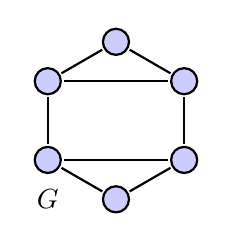
\begin{tikzpicture}[node distance=3cm,
                        thick,main node/.style={circle,fill=blue!20,draw,outer sep=1pt}
                       ]    
      \node[main node] (1) at (0.000,1.000) {};
      \node[main node] (2) at (0.866,0.500) {};
      \node[main node] (3) at (0.866,-0.500) {};
      \node[main node] (4) at (0.00,-1.000) {};
      \node[main node] (5) at (-0.866,-0.500) {};
      \node[main node] (6) at (-0.866,0.500) {};      
       \node (G) at (-0.866,-1.000) {$G$};    
      \path%
        (1) edge node [right] {} (2)  %{} is where the edge value would go
        (2) edge [right] node {} (3)
        (3) edge [right] node {} (4)
        (4) edge [left] node {} (5)
        (5) edge [left] node {} (6)
        (6) edge [left] node {} (1)
        (2) edge [left] node {} (6)
        (3) edge [right] node {} (5);
 \end{tikzpicture}
 \qquad
 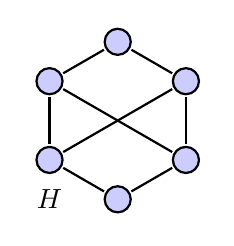
\begin{tikzpicture}[node distance=3cm,
                        thick,main node/.style={circle,fill=blue!20,draw,outer sep=1pt}
                       ]
      \node[main node] (1) at (0.000,1.000) {};
      \node[main node] (2) at (0.866,0.500) {};
      \node[main node] (3) at (0.866,-0.500) {};
      \node[main node] (4) at (0.00,-1.000) {};
      \node[main node] (5) at (-0.866,-0.500) {};
      \node[main node] (6) at (-0.866,0.500) {};      
      \node (G) at (-0.866,-1.000) {$H$};    
      \path%
        (1) edge node [right] {} (2)  %{} is where the edge value would go
        (2) edge [right] node {} (3)
        (3) edge [right] node {} (4)
        (4) edge [left] node {} (5)
        (5) edge [left] node {} (6)
        (6) edge [left] node {} (1)
        (2) edge [left] node {} (5)
        (3) edge [right] node {} (6);
 \end{tikzpicture}
\caption{Nonisomorphic grades with the same degree sequences.}
\end{marginfigure}

\vskip 30pt
For graphs with a few vertices and a few edges, a little trial and error is typically enough to determine if the graphs are isomorphic. For more complicated graphs, it can be very difficult to determine if they are isomorphic or not.  One of the big goals in theoretical computer science is the design of  efficient algorithms to determine if two graphs are isomorphic.    

\begin{exmp}
   \begin{marginfigure}
        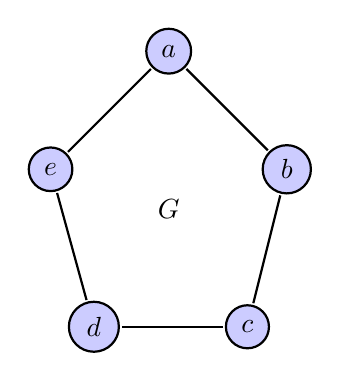
\begin{tikzpicture}[node distance=1cm,
                               thick,main node/.style={circle,fill=blue!20,draw,outer sep=1pt}
                              ]        
             \node[main node] (1) at (0,0) {$e$};
             \node[main node] (2) at (1.5,1.5) {$a$};
             \node[main node] (3) at (3,0) {$b$};
             \node[main node] (4) at (2.5,-2.00) {$c$};
             \node[main node] (5) at (0.55,-2.00) {$d$};
             \node (G) at (1.50,-0.50) {$G$};          
             \path%
               (1) edge node [right] {} (2)  %{} is where the edge value would go
               (2) edge [right] node {} (3)
               (3) edge [right] node {} (4)
               (4) edge [left] node {} (5)
               (5) edge [left] node {} (1);
         \end{tikzpicture}
         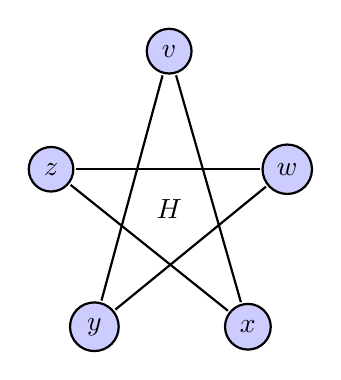
\begin{tikzpicture}[node distance=1cm,
                                 thick,main node/.style={circle,fill=blue!20,draw,outer sep=1pt}
                                ]           
               \node[main node] (1) at (0,0) {$z$};
               \node[main node] (2) at (1.5,1.5) {$v$};
               \node[main node] (3) at (3,0) {$w$};
               \node[main node] (4) at (2.5,-2.00) {$x$};
               \node[main node] (5) at (0.55,-2.00) {$y$};       
               \node (H) at (1.50,-0.50) {$H$};
               \path%
                 (1) edge node [right] {} (3)  %{} is where the edge value would go
                 (3) edge [right] node {} (5)
                 (5) edge [right] node {} (2)
                 (2) edge [left] node {} (4)
                 (4) edge [left] node {} (1);
           \end{tikzpicture}
           \caption{Isomorphic graphs}\label{fig:iso graphs}
      \end{marginfigure}%
  Let $G$ be a 5-cycle on $a,b,c,d,e$ drawn as a regular pentagon
  with vertices
  arranged clockwise, in order, at the corners. Let $H$ have vertex set $v,w,x,y,z$ and graphical 
  presentation as a pentagram (five-pointed star), where the vertices of the graph are the ends of the 
  points of the star, and are arranged clockwise, (see figure~\ref{fig:iso graphs}). \\
  An isomorphism is $a\to v, \; b\to x,\;  c\to z,\;  d\to w,\; e\to y.$ 
\end{exmp}

\vfill\break


\begin{exmp}\label{petersen graph}
 The two graphs in figure~\ref{fig:more iso graphs} are isomorphic as shown by using the relabeling 
 \[
  u_1 \to v_1,\; u_2\to v_2,\; u_3\to v_3,\;
   u_4\to v_4, \; u_5\to v_9,
 \]  
 \[  
    u_6\to v_{10},\; u_7\to  v_5,\; 
   u_8\to v_7,\; u_9\to  v_8,\; u_{10}\to v_6.
 \]
 \begin{figure}
 \resizebox{\textwidth}{!}{%
 \centering
   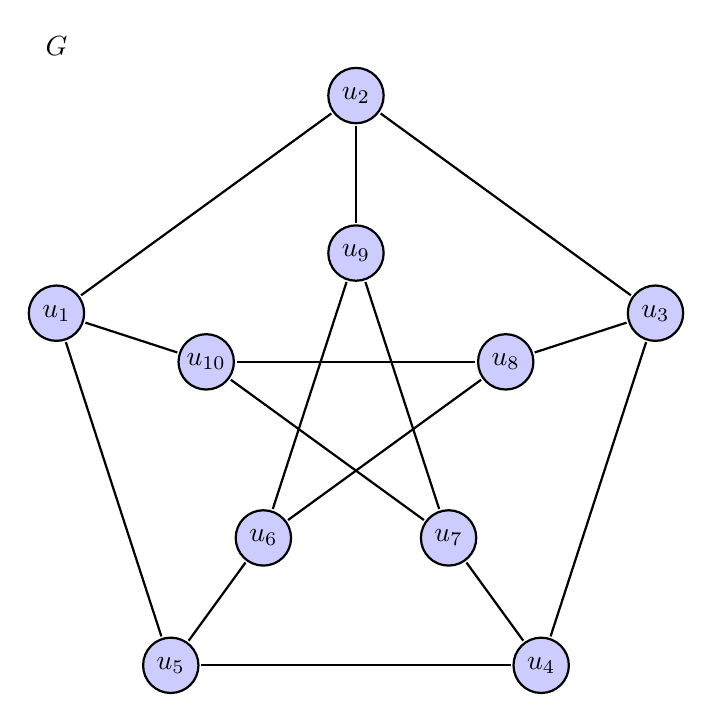
\begin{tikzpicture}[node distance=2cm,
                       thick,main node/.style={circle,fill=blue!20,draw,outer sep=1pt,inner sep=1pt,minimum size=20pt}
                               ]        
              \node[main node] (2) at (0,4) {$u_2$};
              \node[main node] (3) at (3.804,1.236) {$u_3$};
              \node[main node] (4) at (2.352,-3.236) {$u_4$};
              \node[main node] (5) at (-2.352,-3.236) {$u_5$};
              \node[main node] (1) at (-3.804,1.236) {$u_1$};
              \node[main node] (9) at (0,2) {$u_9$};
              \node[main node] (8) at (1.902,0.618) {$u_8$};
              \node[main node] (7) at (1.176,-1.618) {$u_7$};
              \node[main node] (6) at (-1.176,-1.618) {$u_6$};
              \node[main node] (10) at (-1.902,0.618) {$u_{10}$}; 
              \node (G) at (-3.804,4.625) {$G$};        
              \path%
                (1) edge node [right] {} (2)  %{} is where the edge value would go
                (2) edge [right] node {} (3)
                (3) edge [right] node {} (4)
                (4) edge [left] node {} (5)
                (5) edge [left] node {} (1)
                (1) edge [left] node {} (10)
                (2) edge [left] node {} (9)
                (3) edge [left] node {} (8)
                (4) edge [left] node {} (7)
                (5) edge [left] node {} (6)
                (6) edge [left] node {} (8)
                (8) edge [left] node {} (10)
                (10) edge [left] node {} (7)
                (7) edge [left] node {} (9)
                (9) edge [left] node {} (6);                              
          \end{tikzpicture}
         \qquad
          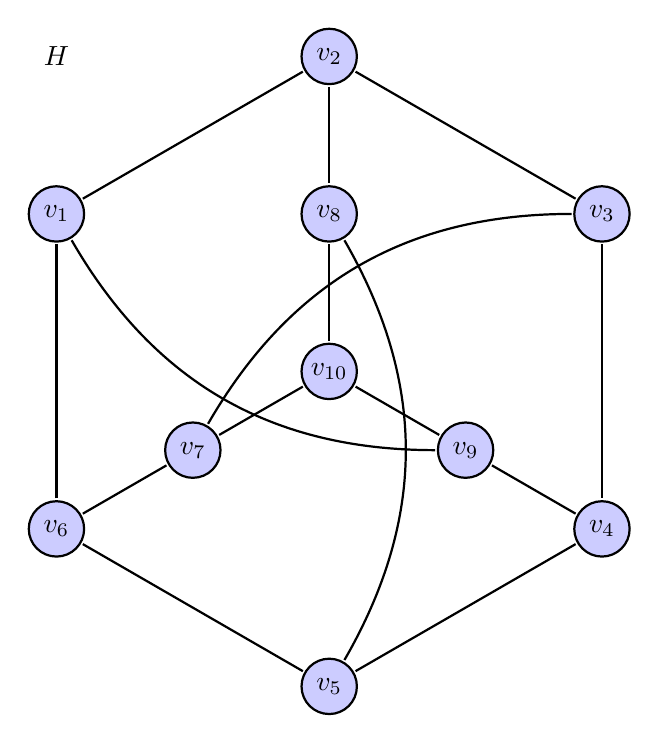
\begin{tikzpicture}[node distance=3cm,
                              thick,main node/.style={circle,fill=blue!20,draw,outer sep=1pt,inner sep=1pt,minimum size=20pt}
                                 ]
                \node[main node] (2) at (0.000,4.000) {$v_2$};
                \node[main node] (3) at (3.464,2.000) {$v_3$};
                \node[main node] (4) at (3.464,-2.000) {$v_4$};
                \node[main node] (5) at (0.00,-4.000) {$v_5$};
                \node[main node] (6) at (-3.464,-2.000) {$v_6$};
                \node[main node] (1) at (-3.464,2.000) {$v_1$};
                \node[main node] (7) at (-1.732,-1.000) {$v_7$};
                \node[main node] (8) at (0.000,2.000) {$v_8$};
                \node[main node] (9) at (1.732,-1.000) {$v_9$};
                \node[main node] (10) at (0.000,0.000) {$v_{10}$};   
                 \node (H) at (-3.464,4.000) {$H$};
                \path%
                  (1) edge node [right] {} (2)  %{} is where the edge value would go
                  (2) edge [right] node {} (3)
                  (3) edge [right] node {} (4)
                  (4) edge [left] node {} (5)
                  (5) edge [left] node {} (6)
                  (6) edge [left] node {} (1)
                  (2) edge [right] node {} (8)
                  (4) edge [right] node {} (9)
                  (6) edge [right] node {} (7)
                  (7) edge [right] node {} (10)
                  (8) edge [right] node {} (10)
                  (9) edge [right] node {} (10)
                  (1) edge [bend right] node {} (9)
                  (3) edge [bend right] node {} (7)
                  (5) edge [bend right] node {} (8);
           \end{tikzpicture}%
        } %end resizebox
    \caption{More Isomorphic graphs}\label{fig:more iso graphs}
 \end{figure}
\end{exmp}
The graph $G$ is the traditional presentation of the {\bfseries {Petersen Graph}}.
It could be described as the graph whose vertex set is labeled with  all the two element subsets of a five element set, with an edge
joining two vertices if their labels have exactly one element in common. 

\section{Paths}\label{sect:paths}

The origins of graph theory had to do with bridges, and possible routes crossing the bridges. In this section we will consider that sort of question in graphs in general. We will think of walking along edges, from one vertex in the list to the next, and visiting vertices. Remember that we do not allow multiple edges or loops in our graphs. 

We begin with a collection of definitions. Warning: These terms are used differently in different texts. If you look at another graph theory text, be sure to see how the terms are used there.

A {\bfseries path} of {\bfseries {length}} $n$ in a graph is a sequence of $n+1$ vertices
$v_0, v_1, v_2,..., v_n$, where each vertex in the list is adjacent to the following vertex. Repeated vertices and repeated edges in a path are allowed.  The vertices $v_0$ and $v_{n}$ are the {\bfseries endpoints} of the path. Think of starting at $v_0$, walking along the edges, and ending up at $v_n$. The length $n$ of the walk is the number of edges transversed in the path.    A path of length three or more for which the endpoints are the same (so $v_0 = v_n$) is called a {\bfseries circuit}. A {\bfseries simple} path (or circuit) is one that does not repeat any edges. A single vertex $v$ will be considered to be a path (but not a circuit!) of length $0$.



Here is an example illustrating these definitions.

\begin{exmp}
 In the graph shown in figure~\ref{fig:paths in a graph}, 
 $a,b,e,c,f,c$ is a path of length $5$. 
 That is an example of an $a,c${-}path, meaning it starts at vertex $a$ and ends at vertex $c$. 
 That path is not simple since the edge ${c,f}$ is repeated. Note that direction does not matter. 
 The vertex sequence $a,b,c,f,e$ is an $a,e${-}path.  Here are two simple circuits in that graph: $a,b,e,d,a$ and $a,b,c,e,d,a$. Notice that the circuit $a,e,b,c,f,e,d,a$ is also simple even though it repeats the vertex $e$. It does not repeat any edges.  
 
\begin{marginfigure}
\resizebox{\textwidth}{!}{%
 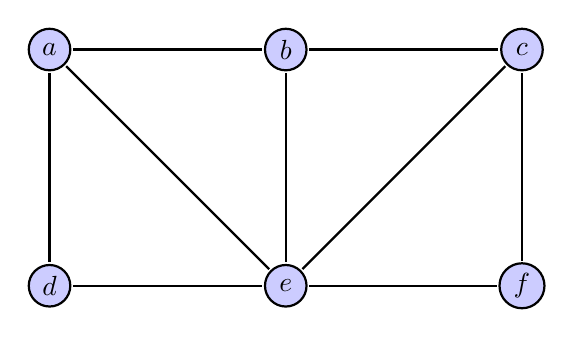
\begin{tikzpicture}[node distance=1cm,
                      thick,main node/.style={circle,fill=blue!20,draw,outer sep=1pt,
                      inner sep=2pt,minimum size=15pt}
                     ]           
   \node[main node] (a) at (0.0,0.0) {$a$};
   \node[main node] (b) at (3.0,0.0) {$b$};
   \node[main node] (c) at (6.0,0.0) {$c$};
   \node[main node] (d) at (0.0,-3.0) {$d$};
   \node[main node] (e) at (3.0,-3.0) {$e$};       
   \node[main node] (f) at (6.0,-3.0) {$f$};
   \path%
     (a) edge node [right] {} (b)  %{} is where the edge value would go
     (b) edge [right] node {} (c)
     (c) edge [right] node {} (f)
     (f) edge [left] node {} (e)
     (e) edge [left] node {} (d)
     (d) edge [left] node {} (a)
     (a) edge [left] node {} (e)
     (b) edge [left] node {} (e)
     (c) edge [left] node {} (e);
\end{tikzpicture}
} %end resizebox
\caption{paths and circuits}\label{fig:paths in a graph}
\end{marginfigure}
\end{exmp} 

A graph is {\bfseries {connected}} if there is a path between any two vertices. In plain English, a connected graph consists of a single piece. The individual connected pieces of a graph are called its {\bfseries connected components}. The length of the shortest path between two vertices in a connect component of a graph is called the {\bfseries distance} between the vertices.  In  figure~\ref{fig:paths in a graph},
the distance between $a$ and $f$ is $2$. 

\begin{thm}\label{thm:exists simple path}
 In a connected graph there is a simple path between
 any two vertices. In other words, if there is a way to get from one vertex to another vertex along edges, then there
 is a way to get between those two vertices without repeating any edges.
\end{thm}
\begin{proof}
Problem~\ref{prob:prove thm simple path}. The idea is simple: in a path with a repeated edge, just eliminate the {\it side trip} made between the two occurrences of that edge from the path. Do that until all the repeated edges are eliminated. For example,  in the graph shown in figure~\ref{fig:paths in a graph}, The $a,c${-}path $a,e,b,e,c$ can be reduced to the path $a,e,c$, eliminating the side trip to $b$.
\end{proof}


A vertex in a graph is a {\bfseries {cut vertex}}, if removal of the vertex and edges incident to it 
results in a graph with more connected components. Similarly a {\bfseries {bridge}} is an edge whose removal (keeping the vertices it is incident to) 
yields a graph with more connected components.

We close this section with a discussion of two special types of paths.

\subsection{Eulerian paths and circuits}

An {\bfseries {eulerian path}} in a graph is a simple path which transverses every edge of the graph. In other words, an eulerian path in a graph is a path that transverses every edge of the graph exactly once. 
An interesting property 
of a graph with an eulerian path is that it can be drawn completely
without lifting pencil from paper and without retracing any edges.

An {\bfseries {eulerian circuit}} is a simple circuit in a graph that transverses every edge of the graph. So an eulerian circuit  is a path of length three or more that transverses every edge of the graph and ends up at its initial vertex.
A graph is called {\bfseries eulerian} if it has an eulerian circuit.

\begin{exmp}
 The graph $C_5$ is an eulerian graph. In fact, the graph itself is an eulerian circuit. 
\end{exmp}


\begin{exmp}
 The graph $K_5$ is an eulerian graph. 
\end{exmp}

\begin{exmp}
 The graph $L_n$ is itself an eulerian path, but does not have an eulerian circuit.
\end{exmp}

\begin{exmp}
 The graph $K_4$ is not an eulerian graph. \sidenote{Try it!}.
\end{exmp}

\subsection{Hamiltonian paths and circuits}

A {\bfseries {hamiltonian path}} in a graph is a simple path that visits every vertex in the graph exactly once.
A {\bfseries {hamiltonian circuit}} in a graph is a simple circuit that, except for the last vertex of the circuit, visits every vertex in the graph exactly once.
A graph is {\bfseries hamiltonian} if it has a hamiltonian circuit.

\begin{exmp}
 $K_n$ is hamiltonian for $n\geq 3$.
\end{exmp} 

\begin{exmp}
 $W_n$ has a hamiltonian circuit for $n\geq 3$.
\end{exmp} 

\begin{exmp}
 $L_n$ has no hamiltonian circuit for $n\geq 2$
\end{exmp} 

\subsection{Some facts about eulerian and hamiltonian graphs}

A few easy observation: if $G$ is a graph with either an eulerian circuit  or hamiltonian
circuit, then
\begin{enumerate}
 \item $G$ is connected.
 
 \item every vertex has degree at least 2.
 
 \item $G$ has no bridges.
 
 \end{enumerate}
 
 If $G$ has a hamiltonian circuit, then $G$ has no cut vertices. 

Leonhard Euler gave a simple way to determine exactly when a graph is eulerian. On the other hand,  despite considerable effort, no one has been able to devise a test to distinguish between hamiltonian and nonhamiltonian graphs that is much better than a brute force trial{-}and{-}error search for a hamiltonian circuit. 

\begin{thm}
 A connected graph is eulerian if and only if  every vertex has even degree.
\end{thm}
\begin{proof}
 Let $G$ be an eulerian graph, and suppose that $v$ is a vertex in 
 $G$ with odd degree, say $2m+1$. Let $i$ denote the number of times an eulerian circuit  passes through 
 $v$. Since every edge is used exactly once in the circuit, and each time $v$ is visited two different edges are used, 
 we have $2i=2m+1$, which is impossible. $\ctrdct$. So $G$ cannot have any vertices of odd degree.
 
 Conversely, let $G$ be a connected graph where every vertex has even degree. 
 Select a vertex $u$ and build  a simple path starting at $u$ as long as possible:
 each time we visit a vertex we select an unused edge leaving that vertex to extend the simple path. For any vertex $v\neq u$ we visit,  its even
 degree guarantees there will be an unused edge out, since each time $v$ is visited used two edges incident to $v$ and one more edge to arrive at $v$, for a total of an odd number of edges incident to $v$, and the vertex has even degree, so there must be at least one unused edge leading out of $v$.
 Since the process of extending the simple path must eventually come to an end, that shows the end must be at $u$ when the simple path cannot be extended, and so we have constructed an eulerian circuit. 
  
 If this simple path contains every edge we are done. Otherwise when these edges are removed from $G$
 we obtain a set of connected components $H_1,...,H_m$ which are subgraphs of $G$ and which
 each satisfy that all vertices have even degree. Since their sizes are smaller, we may inductively
 construct an eulerian circuit for each $H_i$. Since each $G$ is connected, each $H_i$ contains
 a vertex of the initial circuit, say $v_j$. If we call the eulerian circuit of $H_i$, $C_i$, then 
 $v_0,...v_j,C_i,v_j,...,v_n,v_0$ is a circuit in $G$. Since the $H_i$ are disjoint, we may insert each 
 eulerian {\it partial} circuit thus obtaining an eulerian circuit for $G$.
\end{proof} 

As a corollary we have
\begin{thm}
 A connected graph has an eulerian path, but not an eulerian circuit,   if
 and only if
 it has exactly two vertices of odd degree.
\end{thm}

The following theorem is an example of a sufficient (but not necessary) condition for a graph to have a hamiltonian
circuit. 
\begin{thm}
 Let $G$ be a connected graph with $n\geq 3$ vertices. If $deg(v)\geq n/2$
 for every vertex $v$, then $G$ is hamiltonian.
\end{thm}
\begin{proof}
 Suppose that the theorem is false.
 Let $G$ be a connected graph with $deg(v)\geq n/2$
 for every vertex $v$.
 Moreover suppose that of all counterexamples on $n$ vertices, $G$ is a graph with the largest possible number of edges. 
 
 $G$ is not complete, since $K_n$ has a hamiltonian circuit, for $n\geq 3$. Therefore
 $G$ has two nonadjacent vertices $v_1$ and $v_n$. By maximality
 the graph $G_1$ formed by adding the edge $\{v_1,v_n\}$ to $G$ has a hamiltonian circuit. Moreover this circuit uses the
 edge $\{v_1,v_n\}$, since otherwise $G$ has a hamiltonian circuit. So we may suppose that the hamiltonian
 circuit in $G_1$ is of the form $v_1,v_2,...,v_n,v_1$. Thus $v_1,...,v_n$ is a  path
 in $G$.
 
 Let $k=deg(v_1)$. 
 If $v_{i+1}$ is adjacent to $v_1$, then $v_i$ cannot be adjacent to $v_n$, since otherwise $v_1,...,v_i,v_n,v_{n-1},...,v_{i+1},v_1$ is a
 hamiltonian circuit in $G$. Therefore, we have the contradiction
 \[
  deg(v_n)\leq (n-1)-k\leq n-1-n/2=n/2-1.\ctrdct
 \]
\end{proof} 

{\bfseries WARNING}:  Do not read too much into this theorem. The condition is  not a necessary condition. The $5${-}cycle, $C_5$, is obviously hamiltonian, but the vertices all have degree $2$ which is less than $\frac{5}{2}$.

\bigskip

\section{Trees}
Trees form an important class of graphs. A {\bfseries {tree}} is a connected graph with
no circuits.  Trees are traditionally drawn {\it upside down}, with the tree growing down rather than up,  starting at a root vertex.
 
\begin{center}
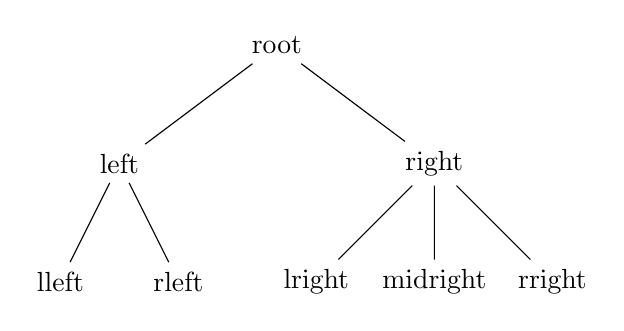
\begin{tikzpicture}[level distance=1.5cm,
  level 1/.style={sibling distance=4cm},
  level 2/.style={sibling distance=1.5cm}]
  \node {root}
    child {node {left}
      child {node {lleft}}
      child {node {rleft}}
    }
    child {node {right}
      child {node {lright}}
      child {node {midright}}
      child {node {rright}}
   };
\end{tikzpicture}
\end{center}

\begin{thm}\label{thm:graph is tree}
 A graph $G$ is a tree if and only if there is a unique path between any two vertices.
\end{thm}
\begin{proof}
 Suppose that $G$ is a tree, and let $u$ and $v$ be two vertices of $G$. Since
 $G$ is connected, there is a path of the form $u=v_0,v_1,...,v_n=v$. 
 If there is a different  path from $u$ to $v$, say $u=w_0,w_1,...,w_n=v$ let $i$ be the smallest subscript
 so that $w_i=v_i$, but $v_{i+1}\neq w_{i+1}$. Also let $j$ be the next smallest subscript where $v_j=w_j$.
 By construction $v_i,v_{i+1},...,v_j,w_{j-1},w_{j-2},...,w_i$ is a circuit in $G \ctrdct$.
 
 Conversely, if $G$ is a graph where there is a unique path between any pair of vertices, then
 by definition $G$ is connected. If $G$ contained a circuit, $C$, then any two vertices of $C$ would be joined
 by two distinct paths.$\ctrdct$ Therefore $G$ contains no circuits, and is a tree.
\end{proof}

A consequence of theorem~\ref{thm:graph is tree} is that given any vertex $r$ in a tree, 
we can draw the tree with $r$ at the
top, as the root vertex,  and the other vertices in levels below. \sidenote {Redraw the tree diagram above with vertex midright as the root vertex.} The neighbors of $r$ that appear at the first level below $r$
are called $r$'s {\bfseries {children}}. The children of $r$'s children are put
in the second level below $r$, and are $r$'s {\bfseries {grandchildren}}. In general the $i$th level consists of those
vertices in the tree which are at distance $i$ from $r$. The result is called a {\bfseries {rooted tree}}. The {\bfseries {height}} of a rooted tree is the maximum level number.

Naturally, besides child and parent, many genealogical terms apply to rooted trees,
and are suggestive of the structure. For example if  a rooted tree
has root $r$, and $v\not{=}r$, the {\bfseries {ancestors}} of $v$ are all vertices on the 
path from $r$ to $v$, including $r$, but excluding $v$. The {\bfseries {descendants}} of a vertex, $w$
consist of all vertices which have $w$ as one of their ancestors. The {\bfseries {subtree rooted at $w$}}
is the rooted tree consisting of $w$, its descendants, and all the required edges. 
A vertex with no children is a {\bfseries {leaf}}, and a vertex with at least one child is called an
{\bfseries {internal vertex}}.

To distinguish rooted trees by breadth, we use the term {\bfseries {$m$-ary}} to mean that any internal
vertex has at most $m$ children. An $m$-ary tree is {\bfseries {full}} if every internal vertex has
exactly $m$ children. When $m=2$, we use the term {\bfseries {binary}}.


\begin{thm}
 A tree on $n$ vertices has $n-1$ edges.
\end{thm}
\begin{proof}
 ({\it by induction on n.})\\
\underbar{Basis}: Let $n = 1$, this is the trivial tree with $0$ edges.  So true the theorem is true for $n = 1$.

\underbar{Inductive Step}:
Suppose that for some $n\geq 1$ every tree with $n$ vertices has $n-1$ edges.
Now suppose $T$ is a tree with $n+1$ vertices. Let $v$ be a leaf of $T$.
If we erase $v$ and the edge leading to it, we are left with a tree with $n$ vertices.
By the inductive hypothesis, this new tree will have $n-1$ edges. Since it has one less edge than the original tree, we conclude $T$ has $n$ edges.
\end{proof}

\clearpage
\section{Exercises}

\begin{exer}
Find a graph isomorphism $\phi: G \to H$. Verify the adjacency preserving property 
by showing the adjacency matrices satisfy $A_G = A_G^\phi$.

\vspace*{2\baselineskip}
\begin{minipage}[b]{0.4\textwidth}
($G$)\quad\linebreak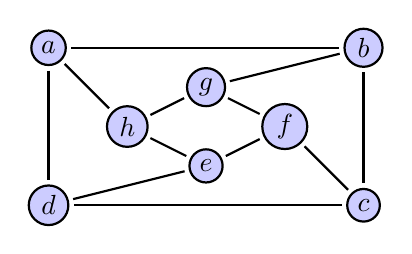
\begin{tikzpicture}[node distance=0.5cm,
                       thick,main node/.style={circle,fill=blue!20,draw,outer sep=2pt,inner sep=2pt}
                      ] 
  \node[main node] (a) at (-2.00,1.00) {$a$};
  \node[main node] (b) at (2.00,1.00) {$b$};
  \node[main node] (c) at (2.00,-1.00) {$c$};
  \node[main node] (d) at (-2.00,-1.00) {$d$};
  \node[main node] (e) at (0.00,-0.50) {$e$};
  \node[main node] (f) at (1.00,0.00) {$f$};
  \node[main node] (g) at (0.00,0.50) {$g$};
  \node[main node] (h) at (-1.00,0.00) {$h$};

  \path%
   (a) edge [left] node {} (b)
   (a) edge [left] node {} (h)
   (a) edge [left] node {} (d)
   (b) edge [left] node {} (c)
   (b) edge [left] node {} (g)
   (c) edge [left] node {} (d)
   (c) edge [left] node {}  (f)
   (d) edge [left] node {} (e)
   (e) edge [left] node {} (f)
   (e) edge [left] node {} (h)
   (g) edge [left] node {} (h)
   (f) edge [left] node {} (g);
 \end{tikzpicture}
\end{minipage}
\hspace*{0.1\textwidth}
\begin{minipage}[b]{0.4\textwidth}
($H$)\quad\linebreak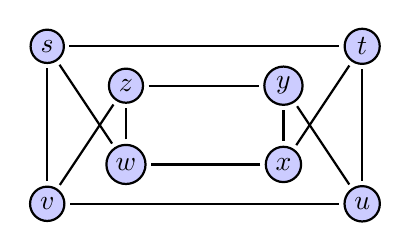
\begin{tikzpicture}[node distance=0.5cm,
                       thick,main node/.style={circle,fill=blue!20,draw,outer sep=2pt,inner sep=2pt}
                      ] 
  \node[main node] (s) at (-2.00,1.00) {$s$};
  \node[main node] (t) at (2.00,1.00) {$t$};
  \node[main node] (u) at (2.00,-1.00) {$u$};
  \node[main node] (v) at (-2.00,-1.00) {$v$};
  \node[main node] (w) at (-1.00,-0.50) {$w$};
  \node[main node] (x) at (1.00,-0.50) {$x$};
  \node[main node] (y) at (1.00,0.50) {$y$};
  \node[main node] (z) at (-1.00,0.50) {$z$};

  \path%
   (s) edge [left] node {} (t)
   (t) edge [left] node {} (u)
   (u) edge [left] node {} (v)
   (v) edge [left] node {} (s)
   (s) edge [left] node {} (w)
   (t) edge [left] node {} (x)
   (u) edge [left] node {} (y)
   (v) edge [left] node {} (z)
   (z) edge [left] node {} (y)
   (y) edge [left] node {} (x)
   (x) edge [left] node {} (w)
   (w) edge [left] node {} (z);
 \end{tikzpicture}
 \end{minipage}
\end{exer}

\begin{exer}
Prove that $G$ and  $H$ are not isomorphic.

\vspace*{2\baselineskip}
\begin{minipage}[b]{0.4\textwidth}
($G$)\quad\linebreak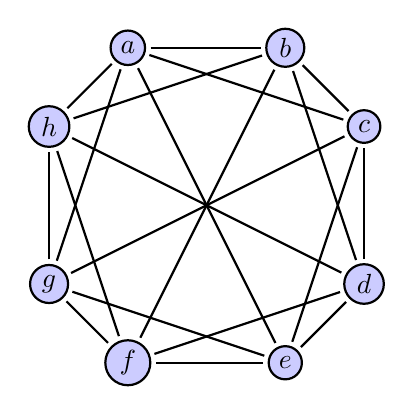
\begin{tikzpicture}[node distance=0.5cm,
                       thick,main node/.style={circle,fill=blue!20,draw,outer sep=2pt,inner sep=2pt}
                      ] 
  \node[main node] (a) at (-1.00,2.00) {$a$};
  \node[main node] (b) at (1.00,2.00) {$b$};
  \node[main node] (c) at (2.00,1.00) {$c$};
  \node[main node] (d) at (2.00,-1.00) {$d$};
  \node[main node] (e) at (1.00,-2.00) {$e$};
  \node[main node] (f) at (-1.00,-2.00) {$f$};
  \node[main node] (g) at (-2.00,-1.00) {$g$};
  \node[main node] (h) at (-2.00,1.00) {$h$};

  \path%
   (a) edge [left] node {} (b)
   (b) edge [left] node {} (c)
   (c) edge [left] node {} (d)
   (d) edge [left] node {} (e)
   (e) edge [left] node {} (f)
   (f) edge [left] node {} (g)
   (g) edge [left] node {} (h)
   (h) edge [left] node {} (a)
   (a) edge [left] node {} (c)
   (a) edge [left] node {} (e)
   (a) edge [left] node {} (g)
   (b) edge [left] node {} (d)
   (b) edge [left] node {} (f)
   (b) edge [left] node {} (h)
   (c) edge [left] node {} (e)
   (c) edge [left] node {} (g)   
   (d) edge [left] node {} (f)
   (d) edge [left] node {} (h)   
   (e) edge [left] node {} (g)
   (f) edge [left] node {} (h);
 \end{tikzpicture}
\end{minipage}
\hspace*{0.1\textwidth}
\begin{minipage}[b]{0.4\textwidth}
($H$)\quad\linebreak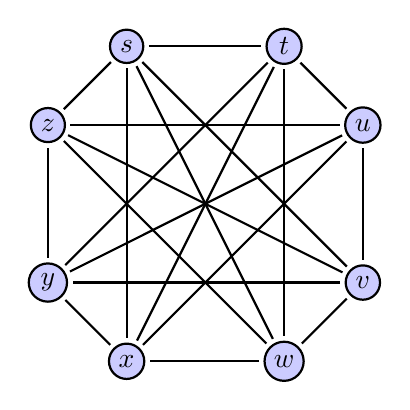
\begin{tikzpicture}[node distance=0.5cm,
                       thick,main node/.style={circle,fill=blue!20,draw,outer sep=2pt,inner sep=2pt}
                      ] 
  \node[main node] (s) at (-1.00,2.00) {$s$};
  \node[main node] (t) at (1.00,2.00) {$t$};
  \node[main node] (u) at (2.00,1.00) {$u$};
  \node[main node] (v) at (2.00,-1.00) {$v$};
  \node[main node] (w) at (1.00,-2.00) {$w$};
  \node[main node] (x) at (-1.00,-2.00) {$x$};
  \node[main node] (y) at (-2.00,-1.00) {$y$};
  \node[main node] (z) at (-2.00,1.00) {$z$};

  \path%
   (s) edge [left] node {} (t)
   (t) edge [left] node {} (u)
   (u) edge [left] node {} (v)
   (v) edge [left] node {} (w)
   (w) edge [left] node {} (x)
   (x) edge [left] node {} (y)
   (y) edge [left] node {} (z)
   (z) edge [left] node {} (s)
   (s) edge [left] node {} (v)
   (s) edge [left] node {} (w)
   (s) edge [left] node {} (x)
   (t) edge [left] node {} (w)
   (t) edge [left] node {} (x)
   (t) edge [left] node {} (y)
   (u) edge [left] node {} (x)
   (u) edge [left] node {} (y)
   (u) edge [left] node {} (z)
   (v) edge [left] node {} (y)
   (v) edge [left] node {} (z)
   (w) edge [left] node {} (z);
   
  \end{tikzpicture}
 \end{minipage}
\end{exer}

\begin{exer}
Redraw the graph $G$ as a bipartite graph.

\vspace*{2\baselineskip}
($G$)\quad\linebreak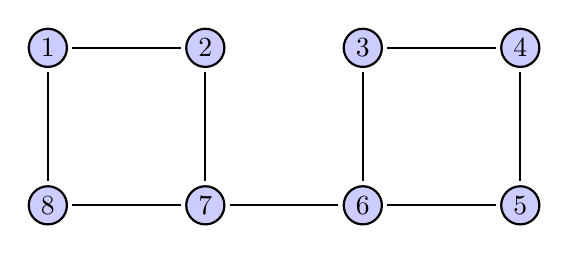
\begin{tikzpicture}[node distance=0.5cm,
                       thick,main node/.style={circle,fill=blue!20,draw,outer sep=2pt,inner sep=2pt}
                      ] 
  \node[main node] (1) at (-3.00,2.00) {$1$};
  \node[main node] (2) at (-1.00,2.00) {$2$};
  \node[main node] (3) at (1.00,2.00) {$3$};
  \node[main node] (4) at (3.00,2.00) {$4$};
  \node[main node] (5) at (3.00,0.00) {$5$};
  \node[main node] (6) at (1.00,0.00) {$6$};
  \node[main node] (7) at (-1.00,0.00) {$7$};
  \node[main node] (8) at (-3.00,0.00) {$8$};

  \path%
   (1) edge [left] node {} (2)
   (3) edge [left] node {} (4)
   (1) edge [left] node {} (8)
   (2) edge [left] node {} (7)
   (3) edge [left] node {} (6)
   (4) edge [left] node {} (5)
   (8) edge [left] node {} (7)
   (7) edge [left] node {} (6)
   (6) edge [left] node {} (5);
 \end{tikzpicture}
\end{exer}

\begin{exer}
Explain why the graph $G$ is not eulerian, but is hamiltonian.
\vspace*{2\baselineskip}
($G$)\quad\linebreak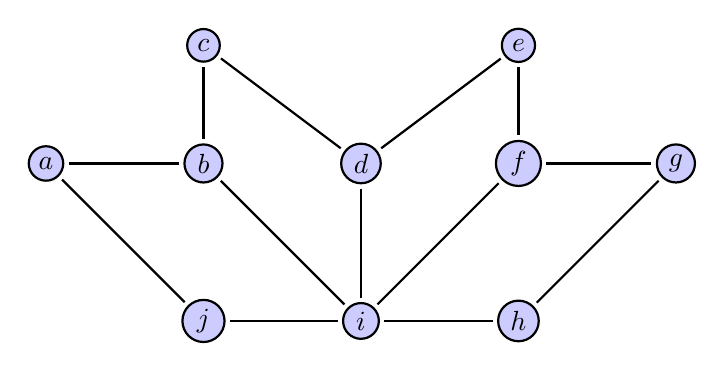
\begin{tikzpicture}[node distance=0.5cm,
                       thick,main node/.style={circle,fill=blue!20,draw,outer sep=2pt,inner sep=2pt}
                      ] 
  \node[main node] (a) at (-4.00,2.00) {$a$};
  \node[main node] (b) at (-2.00,2.00) {$b$};
  \node[main node] (c) at (-2.00,3.50) {$c$};
  \node[main node] (d) at (0.00,2.00) {$d$}; 
  \node[main node] (e) at (2.00,3.50) {$e$};
  \node[main node] (f) at (2.00,2.00) {$f$};
  \node[main node] (g) at (4.00,2.00) {$g$};
  \node[main node] (h) at (2.00,0.00) {$h$};
  \node[main node] (i) at (0.00,0.00) {$i$};
  \node[main node] (j) at (-2.00,0.00) {$j$};

  \path%
   (a) edge [left] node {} (b)
   (b) edge [left] node {} (c)
   (c) edge [left] node {} (d)
   (d) edge [left] node {} (e)
   (e) edge [left] node {} (f)
   (f) edge [left] node {} (g)
   (g) edge [left] node {} (h)
   (h) edge [left] node {} (i)
   (i) edge [left] node {}  (j)
   (j) edge [left] node {} (a)
   (i) edge [left] node {} (b)
   (i) edge [left] node {} (d)
   (i) edge [left] node {} (f);
 \end{tikzpicture}
\end{exer}

\begin{exer}
Find an eulerian circuit for the graph $G$ as a list of vertices.

\vspace*{2\baselineskip}

($G$)\quad\linebreak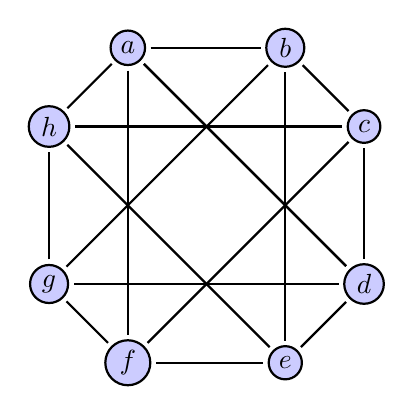
\begin{tikzpicture}[node distance=0.5cm,
                       thick,main node/.style={circle,fill=blue!20,draw,outer sep=2pt,inner sep=2pt}
                      ] 
  \node[main node] (a) at (-1.00,2.00) {$a$};
  \node[main node] (b) at (1.00,2.00) {$b$};
  \node[main node] (c) at (2.00,1.00) {$c$};
  \node[main node] (d) at (2.00,-1.00) {$d$};
  \node[main node] (e) at (1.00,-2.00) {$e$};
  \node[main node] (f) at (-1.00,-2.00) {$f$};
  \node[main node] (g) at (-2.00,-1.00) {$g$};
  \node[main node] (h) at (-2.00,1.00) {$h$};

  \path%
   (a) edge [left] node {} (b)
   (b) edge [left] node {} (c)
   (c) edge [left] node {} (d)
   (d) edge [left] node {} (e)
   (e) edge [left] node {} (f)
   (f) edge [left] node {} (g)
   (g) edge [left] node {} (h)
   (h) edge [left] node {} (a)
   (a) edge [left] node {} (d)
   (a) edge [left] node {} (f)
   (b) edge [left] node {} (e)
   (b) edge [left] node {} (g)
   (c) edge [left] node {} (f)
   (c) edge [left] node {} (h)   
   (d) edge [left] node {} (g)
   (d) edge [left] node {} (a)   
   (e) edge [left] node {} (h);
 \end{tikzpicture}
\end{exer}

\begin{exer}
Prove that the graph $G$ has no hamiltonian circuit.

\vspace*{2\baselineskip}
($G$)\quad\linebreak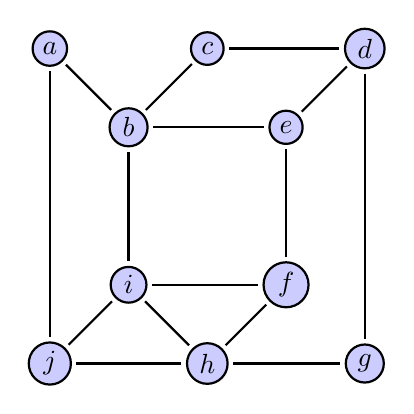
\begin{tikzpicture}[node distance=0.5cm,
                       thick,main node/.style={circle,fill=blue!20,draw,outer sep=2pt,inner sep=2pt}
                      ] 
  \node[main node] (a) at (-2.00,4.00) {$a$};
  \node[main node] (b) at (-1.00,3.00) {$b$};
  \node[main node] (c) at (0.00,4.00) {$c$};
  \node[main node] (d) at (2.0,4.00) {$d$};
  \node[main node] (e) at (1.00,3.00) {$e$};
  \node[main node] (f) at (1.00,1.00) {$f$};
  \node[main node] (g) at (2.0,0.00) {$g$};
  \node[main node] (h) at (0.00,0.00) {$h$};
  \node[main node] (i) at (-1.00,1.00) {$i$};
  \node[main node] (j) at (-2.00,0.00) {$j$};

  \path%
   (a) edge [left] node {} (b)
   (b) edge [left] node {} (c)
   (c) edge [left] node {} (d)
   (d) edge [left] node {} (g)
   (g) edge [left] node {} (h)
   (h) edge [left] node {} (j)
   (j) edge [left] node {} (a)
   (d) edge [left] node {} (e)
   (h) edge [left] node {} (f)
   (h) edge [left] node {} (i)
   (j) edge [left] node {} (i)
   (b) edge [left] node {} (e)
   (e) edge [left] node {} (f)
   (f) edge [left] node {} (i)
   (i) edge [left] node {} (b);
 \end{tikzpicture}
\end{exer}


\clearpage
\section{Problems}

\begin{prob}
\
 \begin{enumerate}[label = (\alph*)]
\item How many edges are there in $K_n$, the complete graph with $n$ vertices?
\item How many edges are there in $C_n$, the $n${-}cycle with $n$ vertices?
\item How many edges are there in $L_n$, the $n${-}link with $n$ vertices?
\item How many edges are there in $W_n$, the $n${-}wheel with $n+1$ vertices?
\item How many edges are there in $Q_n$, the $n${-}cube with $2^n$  vertices?
\item How many edges are there in $K_{m,n}$, the complete bipartite graph with $m$ {\itshape top} and $n$ {\itshape bottom} vertices?
\end{enumerate}
\end{prob}

\begin{prob}\label{prob:bipartite graphs}
Determine whether each graph is bipartite. If it is, redraw it as a bipartite graph.

\vspace*{\baselineskip}
\begin{minipage}[b]{0.4\textwidth}
(a)\quad\linebreak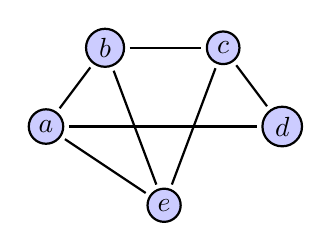
\begin{tikzpicture}[node distance=0.5cm,
                       thick,main node/.style={circle,fill=blue!20,draw,outer sep=2pt,inner sep=2pt}
                      ] 
  \node[main node] (a) at (-1.5,0) {$a$};
  \node[main node] (b) at (-0.75,1.00) {$b$};
  \node[main node] (c) at (0.75,1.00) {$c$};
  \node[main node] (d) at (1.5,0) {$d$};
  \node[main node] (e) at (0,-1.00) {$e$};
  \path%
   (a) edge [left] node {} (b)
   (a) edge [left] node {} (d)
   (a) edge [left] node {} (e)
   (b) edge [left] node {} (c)
   (b) edge [left] node {} (e)
   (c) edge [left] node {} (d)
   (c) edge [left] node {} (e);
 \end{tikzpicture}
\end{minipage}
\hspace*{0.1\textwidth}
\begin{minipage}[b]{0.4\textwidth}
 (b)\quad\linebreak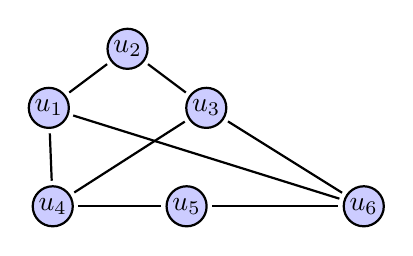
\begin{tikzpicture}[node distance=1cm,
                     thick,main node/.style={circle,fill=blue!20,draw,outer sep=2pt,inner sep=1pt}
                    ]        
   \node[main node] (u1) at (0,0) {$u_1$};
   \node[main node] (u2) at (1,0.75) {$u_2$};
   \node[main node] (u3) at (2.0,0) {$u_3$};
   \node[main node] (u5) at (1.75,-1.25) {$u_5$};
   \node[main node] (u4) at (0.05,-1.25) {$u_4$};
   \node[main node] (u6) at (4.00,-1.25) {$u_6$};       
   \path%
     (u1) edge node [right] {} (u2)  %{} is where the edge value would go
     (u2) edge [right] node {} (u3)
     (u3) edge [right] node {} (u4)
     (u4) edge [left] node {} (u1)
     (u1) edge [left] node {} (u6)
     (u4) edge [left] node {} (u5)
     (u5) edge [left] node {} (u6)
     (u3) edge [left] node {} (u6);
 \end{tikzpicture}
\end{minipage}

\vspace*{\baselineskip}
\begin{minipage}[b]{0.4\textwidth}
(c)\quad\linebreak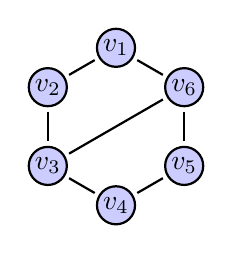
\begin{tikzpicture}[node distance=3cm,
                    thick,main node/.style={circle,fill=blue!20,draw,outer sep=2pt,inner sep=1pt}
                   ]  
  \node[main node] (v1) at (0.000,1.000) {$v_1$};
  \node[main node] (v6) at (0.866,0.500) {$v_6$};
  \node[main node] (v5) at (0.866,-0.500) {$v_5$};
  \node[main node] (v4) at (0.00,-1.000) {$v_4$};
  \node[main node] (v3) at (-0.866,-0.500) {$v_3$};
  \node[main node] (v2) at (-0.866,0.500) {$v_2$};          
  \path%
    (v1) edge node [right] {} (v2)  %{} is where the edge value would go
    (v2) edge [right] node {} (v3)
    (v3) edge [right] node {} (v4)
    (v4) edge [left] node {} (v5)
    (v5) edge [left] node {} (v6)
    (v6) edge [left] node {} (v1)
    (v3) edge [right] node {} (v6);
\end{tikzpicture}
\end{minipage}
\hspace*{0.1\textwidth}
\begin{minipage}[b]{0.4\textwidth}
 (d)\quad\linebreak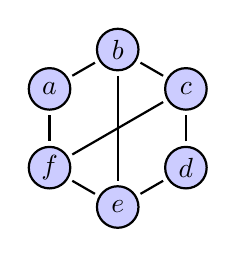
\begin{tikzpicture}[node distance=3cm,
                     thick,main node/.style={circle,fill=blue!20,draw,outer sep=2pt,inner sep=1pt,minimum size=15pt}
                    ]  
   \node[main node] (b) at (0.000,1.000) {$b$};
   \node[main node] (c) at (0.866,0.500) {$c$};
   \node[main node] (d) at (0.866,-0.500) {$d$};
   \node[main node] (e) at (0.00,-1.000) {$e$};
   \node[main node] (f) at (-0.866,-0.500) {$f$};
   \node[main node] (a) at (-0.866,0.500) {$a$};          
   \path%
     (b) edge node [right] {} (a)  %{} is where the edge value would go
     (a) edge [right] node {} (f)
     (f) edge [right] node {} (e)
     (e) edge [left] node {} (d)
     (d) edge [left] node {} (c)
     (c) edge [left] node {} (b)
     (f) edge [right] node {} (c)
     (b) edge [right] node {} (e);
 \end{tikzpicture}
\end{minipage}

\end{prob}


\begin{prob}
\ 
 \begin{enumerate}[label = (\alph*)]
 \item For which values of $n$ is $C_n$ bipartite?\\[-3pt]
 \item For which values of $n$ is $Q_n$ bipartite?
\end{enumerate}
\end{prob}

\vfill\break

\begin{prob}
Draw the Petersen graph with vertices labeled with the ten different subsets of the five element set $\{a,b,c,d,e\}$ as suggested in example\ref{petersen graph}.
\end{prob}

\begin{prob}
 For the graph below
 \begin{enumerate}
  \item  Determine all the bridges.
  \item  Determine all the cut vertices.
 \end{enumerate}
 
 
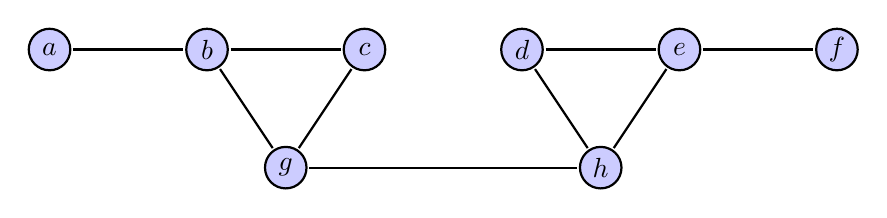
\begin{tikzpicture}[thick,
                       main node/.style={circle,fill=blue!20,draw,outer sep=1pt,
                                         inner sep=1pt,minimum size=15pt}
                      ] 
   \node[main node] (a) at (0.0,3.0) {$a$};
   \node[main node] (b) at (2.0,3.0) {$b$};
   \node[main node] (c) at (4.0,3.0) {$c$};
   \node[main node] (d) at (6.0,3.0) {$d$};
   \node[main node] (e) at (8.0,3.0) {$e$};
   \node[main node] (f) at (10.0,3.0) {$f$};
   \node[main node] (g) at (3.0,1.5) {$g$};
   \node[main node] (h) at (7.0,1.5) {$h$};
   
   \path%
    (a) edge [left] node {} (b)
    (b) edge [left] node {} (c)
    (d) edge [left] node {} (e)
    (e) edge [left] node {} (f)
    (b) edge [left] node {} (g)
    (c) edge [left] node {} (g)
    (d) edge [left] node {} (h)
    (g) edge [left] node {} (h)
    (e) edge [left] node {} (h);
  \end{tikzpicture}
\end{prob}  


\begin{prob} 
For each candidate degree sequence below, either draw a graph with that degree sequence or explain why that list cannot be the degree sequence of a graph.

\begin{enumerate}
\item $4,4,4,4,4$   
\item $6,4,4,4,4$   
\item $0,0,0,0,0$   
\item $3,2,1,1,1$   
\item $3,3,2,2,1$   
\end{enumerate}
\end{prob}

\vfill\break

\begin{prob}
 For each pair of graphs either prove that $G_1$ and $G_2$ are not isomorphic, or else show they are isomorphic by exhibiting a graph isomorphism.
 
\vspace*{\baselineskip}
\begin{minipage}[b]{0.5\textwidth}
(a)\quad\linebreak
 %   \includegraphics{./Graphics/exer38-3-a.pdf}
%% exer38-3-a
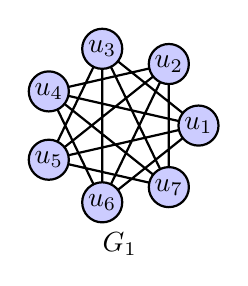
\begin{tikzpicture}[scale=.5,thick, outer sep=0pt,inner sep=1pt]
    \def \N {7}
    \def \radius {2}
    \foreach [count=\x] \k in {1,2,...,\N}
        \node[black, circle,fill=blue!20, draw] (p\x) at ({360/\N * (\k - 1)}:\radius) {$u_{\x}$};

    \draw \foreach \x [remember=\x as \lastx (initially 1)] in {3,5,7,2,4,6,1}{(p\lastx) -- (p\x)};
     \draw \foreach \x [remember=\x as \lastx (initially 1)] in {4,7,3,6,2,5,1}{(p\lastx) -- (p\x)};
\node (G1) at (0,-3.00) {$G_1$};     
\end{tikzpicture}
\quad
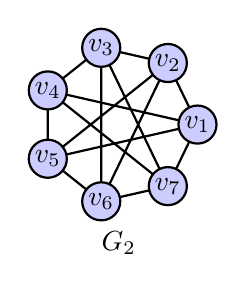
\begin{tikzpicture}[scale=.5,thick, outer sep=0pt,inner sep=1pt]
    \def \N {7}
    \def \radius {2}
    \foreach [count=\x] \k in {1,...,\N}
        \node[black, circle, fill=blue!20, draw] (p\x) at ({360/\N * (\k - 1)}:2) {$v_{\x}$};

    \draw \foreach \x [remember=\x as \lastx (initially 1)] in {4,7,3,6,2,5,1}{(p\lastx) -- (p\x)};
     \draw \foreach \x [remember=\x as \lastx (initially 1)] in {2,3,...,\N,1}{(p\lastx) -- (p\x)}; 
   \node (G2) at (0,-3.00) {$G_2$};
\end{tikzpicture} 
\end{minipage}
\hspace*{0.15\textwidth}
\begin{minipage}[b]{0.6\textwidth}
 (b)\quad\linebreak
%    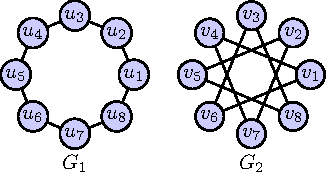
\includegraphics{./Graphics/exer38-3-b.pdf}
% exer38-3-b
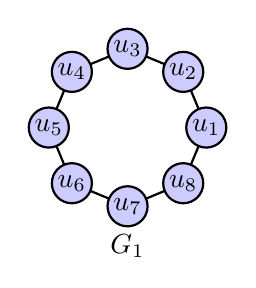
\begin{tikzpicture}[scale=.5,thick, outer sep=0pt,inner sep=1pt]
    \foreach [count=\x] \k in {1,2,...,8}
        \node[black, circle,fill=blue!20, draw] (p\x) at ({360/8 * (\k - 1)}:2) {$u_{\x}$};

    \draw \foreach \x [remember=\x as \lastx (initially 1)] in {2,3,...,8,1}{(p\lastx) -- (p\x)};
    \node (G1) at (0,-3.00) {$G_1$};      
\end{tikzpicture}
\quad
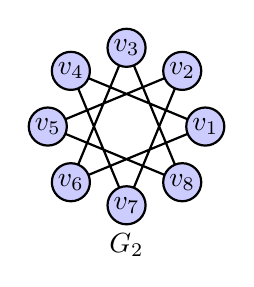
\begin{tikzpicture}[scale=.5,thick, outer sep=0pt,inner sep=1pt]
    \foreach [count=\x] \k in {1,...,8}
        \node[black, circle, fill=blue!20, draw] (p\x) at ({360/8 * (\k - 1)}:2) {$v_{\x}$};

    \draw \foreach \x [remember=\x as \lastx (initially 1)] in {4,7,2,5,8,3,6,1}{(p\lastx) -- (p\x)};
    \node (G2) at (0,-3.00) {$G_2$};
\end{tikzpicture}
\end{minipage}

\vspace*{\baselineskip}
\begin{minipage}[b]{0.5\textwidth}
(c)\quad\linebreak
%   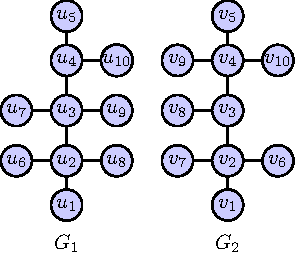
\includegraphics{./Graphics/exer38-3-c.pdf}
%% exer38-3-c
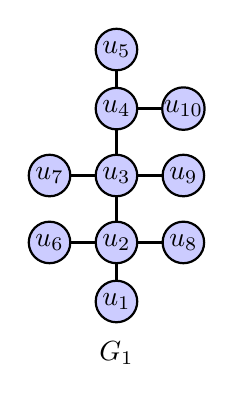
\begin{tikzpicture}[scale=.5,thick, outer sep=0pt,inner sep=0pt,minimum size=15pt]
    \node[black, circle,fill=blue!20, draw] (u1) at (0,-3.2) {$u_1$};
    \node[black, circle,fill=blue!20, draw] (u2) at (0,-1.7) {$u_2$};
    \node[black, circle,fill=blue!20, draw] (u3) at (0,0)  {$u_3$};
    \node[black, circle,fill=blue!20, draw] (u4) at (0,1.7)  {$u_4$};
    \node[black, circle,fill=blue!20, draw] (u5) at (0,3.2)  {$u_5$};
    \node[black, circle,fill=blue!20, draw] (u6) at (-1.7,-1.7) {$u_6$};
    \node[black, circle,fill=blue!20, draw] (u7) at (-1.7,0)  {$u_7$};
    \node[black, circle,fill=blue!20, draw] (u8) at (1.7,-1.7)  {$u_8$};
    \node[black, circle,fill=blue!20, draw] (u9) at (1.7,0)   {$u_9$};
    \node[black, circle,fill=blue!20, draw] (u10) at (1.7,1.7)  {$u_{10}$};
    \path%
      (u1) edge [left] node {} (u2)
      (u2) edge [left] node {} (u3)
      (u3) edge [left] node {} (u4)
      (u4) edge [left] node {} (u5)
      (u2) edge [left] node {} (u6)
      (u2) edge [left] node {} (u8)
      (u3) edge [left] node {} (u7)
      (u3) edge [left] node {} (u9)
      (u4) edge [left] node {} (u10);
   \node (G1) at (0,-4.5) {$G_1$};
\end{tikzpicture}
\quad
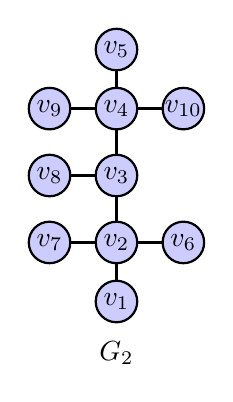
\begin{tikzpicture}[scale=.5,thick, outer sep=0pt,inner sep=0pt,minimum size=15pt]
    \node[black, circle,fill=blue!20, draw] (v1) at (0,-3.2) {$v_1$};
    \node[black, circle,fill=blue!20, draw] (v2) at (0,-1.7) {$v_2$};
    \node[black, circle,fill=blue!20, draw] (v3) at (0,0)  {$v_3$};
    \node[black, circle,fill=blue!20, draw] (v4) at (0,1.7)  {$v_4$};
    \node[black, circle,fill=blue!20, draw] (v5) at (0,3.2)  {$v_5$};
    \node[black, circle,fill=blue!20, draw] (v7) at (-1.7,-1.7) {$v_7$};
    \node[black, circle,fill=blue!20, draw] (v8) at (-1.7,0)  {$v_8$};
    \node[black, circle,fill=blue!20, draw] (v6) at (1.7,-1.7)  {$v_6$};
    \node[black, circle,fill=blue!20, draw] (v10) at (1.7,1.7)   {$v_{10}$};
    \node[black, circle,fill=blue!20, draw] (v9) at (-1.7,1.7)  {$v_{9}$};
    \path%
      (v1) edge [left] node {} (v2)
      (v2) edge [left] node {} (v3)
      (v3) edge [left] node {} (v4)
      (v4) edge [left] node {} (v5)
      (v2) edge [left] node {} (v6)
      (v3) edge [left] node {} (v8)
      (v2) edge [left] node {} (v7)
      (v4) edge [left] node {} (v9)
      (v4) edge [left] node {} (v10);
   \node (G2) at (0,-4.5) {$G_2$};
\end{tikzpicture}
\end{minipage}
\hspace*{0.15\textwidth}
\begin{minipage}[b]{0.6\textwidth}
 (d)\quad\linebreak
%    \includegraphics{./Graphics/exer38-3-d.pdf}
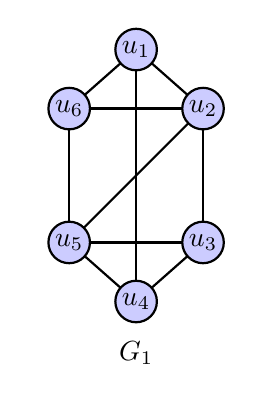
\begin{tikzpicture}[scale=.5,thick, outer sep=0pt,inner sep=0pt,minimum size=15pt]
    \node[black, circle,fill=blue!20, draw] (u1) at (0,3.2) {$u_1$};
    \node[black, circle,fill=blue!20, draw] (u2) at (1.7,1.7) {$u_2$};
    \node[black, circle,fill=blue!20, draw] (u3) at (1.7,-1.7)  {$u_3$};
    \node[black, circle,fill=blue!20, draw] (u4) at (0,-3.2)  {$u_4$};
    \node[black, circle,fill=blue!20, draw] (u5) at (-1.7,-1.7)  {$u_5$};
    \node[black, circle,fill=blue!20, draw] (u6) at (-1.7,1.7) {$u_6$};
    \path%
      (u1) edge [left] node {} (u2)
      (u2) edge [left] node {} (u3)
      (u3) edge [left] node {} (u4)
      (u4) edge [left] node {} (u5)
      (u5) edge [left] node {} (u6)
      (u6) edge [left] node {} (u1)
      (u1) edge [left] node {} (u4)
      (u2) edge [left] node {} (u6)
      (u2) edge [left] node {} (u5)
      (u3) edge [left] node {} (u5);
   \node (G1) at (0,-4.5) {$G_1$};
\end{tikzpicture}
\quad
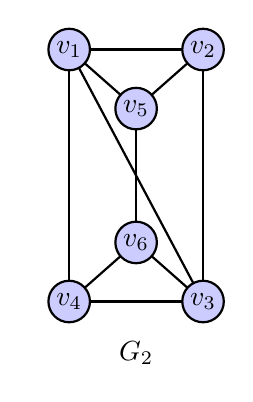
\begin{tikzpicture}[scale=.5,thick, outer sep=0pt,inner sep=0pt,minimum size=15pt]
    \node[black, circle,fill=blue!20, draw] (v1) at (-1.7,3.2) {$v_1$};
    \node[black, circle,fill=blue!20, draw] (v2) at (1.7,3.2) {$v_2$};
    \node[black, circle,fill=blue!20, draw] (v3) at (1.7,-3.2)  {$v_3$};
    \node[black, circle,fill=blue!20, draw] (v4) at (-1.7,-3.2)  {$v_4$};
    \node[black, circle,fill=blue!20, draw] (v5) at (0,1.7)  {$v_5$};
    \node[black, circle,fill=blue!20, draw] (v6) at (0,-1.7)  {$v_6$};
    \path%
      (v1) edge [left] node {} (v2)
      (v2) edge [left] node {} (v3)
      (v3) edge [left] node {} (v4)
      (v4) edge [left] node {} (v1)
      (v1) edge [left] node {} (v5)
      (v2) edge [left] node {} (v5)
      (v3) edge [left] node {} (v6)
      (v4) edge [left] node {} (v6)
      (v5) edge [left] node {} (v6)
      (v1) edge [right] node {} (v3);
   \node (G2) at (0,-4.5) {$G_2$};
\end{tikzpicture}
\end{minipage}
\end{prob}


\begin{prob}\label{prob:prove thm simple path}
 Prove theorem~\ref{thm:exists simple path} from section~\ref{sect:paths}
 on paths:
 \emph{If $G$ is a connected graph, then there is a simple path between
  any two different vertices.}
\end{prob}

\vfill\break

\begin{prob}
 For each graph below
 \begin{enumerate*}[label=(\roman*)]
  \item  find an eulerian circuit, or prove that none exists, and 
  \item  find a hamiltonian circuit or prove that none exists.
 \end{enumerate*}
  
\begin{enumerate}[label=(\alph*),itemsep=0.5cm]
  \item The $3$-cube $Q_3$.
 
 \item
 \ \linebreak
 \begin{minipage}{0.5\textwidth}
  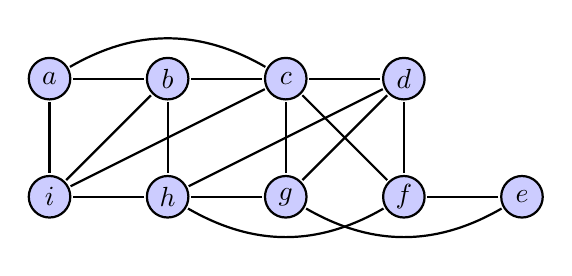
\begin{tikzpicture}[thick,main node/.style={circle,fill=blue!20,draw,outer sep=1pt,inner sep=1pt,minimum size=15pt}
                      ]  
   \node[main node] (a) at (0,1.5) {$a$};
   \node[main node] (b) at (1.5,1.5) {$b$};
   \node[main node] (c) at (3.0,1.5) {$c$};
   \node[main node] (d) at (4.5,1.5) {$d$};
   \node[main node] (i) at (0,0) {$i$};
   \node[main node] (h) at (1.5,0) {$h$};
   \node[main node] (g) at (3.0,0) {$g$};
   \node[main node] (f) at (4.5,0) {$f$};
   \node[main node] (e) at (6.0,0) {$e$};
   \path%
    (a) edge [left] node {} (b)
    (a) edge [bend left] node  {} (c)
    (a) edge [left] node {} (i)
    (b) edge [left] node {} (c)
    (b) edge [left] node {} (h)
    (b) edge [left] node {} (i)
    (c) edge [left] node {} (d)
    (c) edge [left] node {} (f)
    (c) edge [left] node {} (g)
    (c) edge [left] node {} (i)
    (d) edge [left] node {} (f)
    (d) edge [left] node {} (g)
    (d) edge [left] node {} (h)
    (e) edge [left] node {} (f)
    (e) edge [bend left] node {} (g)
    (f) edge [bend left] node {} (h)
    (g) edge [left] node {} (h)
    (h) edge [left] node {} (i);
  \end{tikzpicture}
 \end{minipage}
 %\clearpage
 \item
 \ \linebreak
 \begin{minipage}{0.5\textwidth}
  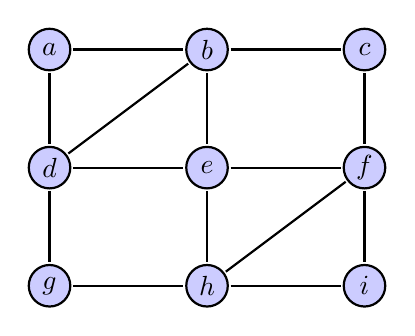
\begin{tikzpicture}[thick,
                       main node/.style={circle,fill=blue!20,draw,outer sep=1pt,
                                         inner sep=1pt,minimum size=15pt}
                      ] 
   \node[main node] (a) at (0.0,3.0) {$a$};
   \node[main node] (b) at (2.0,3.0) {$b$};
   \node[main node] (c) at (4.0,3.0) {$c$};
   \node[main node] (d) at (0.0,1.5) {$d$};
   \node[main node] (e) at (2.0,1.5) {$e$};
   \node[main node] (f) at (4.0,1.5) {$f$};
   \node[main node] (g) at (0.0,0.0) {$g$};
   \node[main node] (h) at (2.0,0.0) {$h$};
   \node[main node] (i) at (4.0,0.0) {$i$};
   \path%
    (a) edge [left] node {} (b)
    (a) edge [left] node {} (d)
    (b) edge [left] node {} (c)
    (b) edge [left] node {} (e)
    (b) edge [left] node {} (d)
    (c) edge [left] node {} (f)
    (d) edge [left] node {} (e)
    (d) edge [left] node {} (g)
    (e) edge [left] node {} (f)
    (e) edge [left] node {} (h)
    (f) edge [left] node {} (h)
    (f) edge [left] node {} (i)
    (g) edge [left] node {} (h)
    (h) edge [left] node {} (i);
  \end{tikzpicture}
 \end{minipage}
 
  \item The Petersen Graph. (See figure~\ref{fig:more iso graphs}.)

\end{enumerate}

\end{prob}

\begin{prob}
A {\it forest} is a graph consisting of one or more (separate) trees. If the total number of vertices in a forest is $f$, and the number of trees in the forest is $t$, what is the total number of edges in the forest?
\end{prob}

\begin{prob}
A tree is called {\bf star{-}like} if there is exactly one vertex with degree greater than $2$. How many different (that it, nonisomorphic) star{-}like trees are there with six vertices? (Note: If you draw the graph with the vertex of of degree greater than $2$ having the {\it arms} of the tree radiating out from it like spokes on a wheel, the name star{-}like will make sense.)
\end{prob}

\vfill\break

\begin{prob}\label{prob: rooted tree}
 Answer the following questions about the rooted tree shown in figure~\ref{fig:prob rooted tree}. 
 %(on page~\pageref{fig:prob rooted tree}.)
 
 \vspace*{0.25cm}
 \begin{minipage}{0.55\textwidth}
  \begin{enumerate}[label=(\alph*)]
    \item Which vertex is the root?
    \item Which vertices are internal?
    \item Which vertices are leaves?
    \item Which vertices are children of $b$?
    \item Which vertices are grandchildren of $b$?
  \end{enumerate}
  \end{minipage}
  \quad
 \begin{minipage}{0.55\textwidth}
  \begin{enumerate}[label=(\alph*)]\setcounter{enumi}{5}
    \item Which vertex is the parent of $m$?
    \item Which vertices are siblings of $q$?
    \item Which vertices are ancestors of $p$? 
    \item  Which vertices are descendants of $d$?
    \item  What level is $i$ at?
  \end{enumerate}  
 \end{minipage}

 \begin{figure}
  \centering
  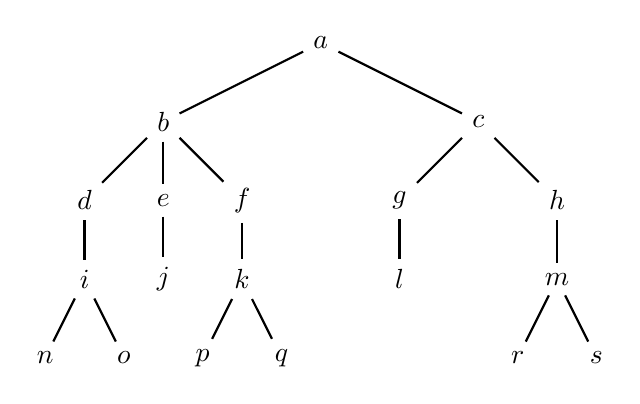
\begin{tikzpicture}[thick]
   \node (root) at (0,0) {$a$};
   \node (l) at (-2.00,-1) {$b$};
   \node (ll) at (-3.00,-2) {$d$};
   \node (llm) at (-3.00,-3) {$i$};
   \node (llml) at (-3.50,-4) {$n$};
   \node (llmr) at (-2.50,-4) {$o$};
   \node (lm) at (-2.00,-2) {$e$};
   \node (lmm) at (-2.00,-3) {$j$};
   \node (lr) at (-1.00,-2) {$f$};
   \node (lrm) at (-1.00,-3) {$k$};
   \node (lrml) at (-1.50,-4) {$p$};
   \node (lrmr) at (-0.50, -4) {$q$};
   \node (r) at (2.00,-1) {$c$};
   \node (rl) at (1.00,-2) {$g$};
   \node (rlm) at (1.00,-3) {$l$};
   \node (rr) at (3.00,-2) {$h$};
   \node (rrm) at (3.00,-3) {$m$};
   \node (rrml) at (2.50,-4) {$r$};
   \node (rrmr) at (3.50,-4) {$s$};
   \path%
     (root) edge [left] node {} (l) %a to b
     (l) edge [left] node {} (ll) %b to d
     (ll) edge [left] node {} (llm) %d to i
     (llm) edge [left] node {} (llml) %i to n
     (llm) edge [left] node {} (llmr) %i to o
     (l) edge [left] node {} (lm) %b to e
     (lm) edge [left] node {} (lmm) %e to j
     (l) edge [left] node {} (lr) %b to f
     (lr) edge [left] node {} (lrm) %f to k
     (lrm) edge [left] node {} (lrml) %k to p
     (lrm) edge [left] node {} (lrmr) %k to q
     (root) edge [left] node {} (r) %root to c
     (r) edge [left] node {} (rl) %c to g
     (rl) edge [left] node {} (rlm) %g to l
     (r) edge [left] node {} (rr) %c to h
     (rr) edge [left] node {} (rrm) %h to m
     (rrm) edge [left] node {} (rrml) %m to r
     (rrm) edge [left] node {} (rrmr); %m to s
   \end{tikzpicture}%
  \caption{Tree for problem~\ref{prob: rooted tree}}\label{fig:prob rooted tree}
 \end{figure}
\end{prob}


